\documentclass{99-Styles/MICE}
\usepackage{bm} % For formatting math mode in bold
\usepackage{amsmath}
\usepackage{graphicx}

%
\input 99-Styles/GetPackages

\linenumbers
\modulolinenumbers[5]
\begin{document}

\input 00a-Top-matter/00a-Top-matter

%\makeatletter

\input 99-Styles/MICE-defs

\parindent 10pt
\pagestyle{plain}
\pagenumbering{arabic}                   
\setcounter{page}{1}

\input 00b-Abstract/00b-Abstract
\section{The MICE Experiment}
\label{sec:MICE}
  \subsection{Overview}
  \label{subsec:Overview}
  The Muon Ionization Cooling Experiment (MICE) will be the first pratical demonstration of ionization cooling of muons. Cooling refers to a reduction in the emittance of a beam, that is, the phase space volume occupied. Beam cooling is required for any future facility based on high intensity muon beams, such as a Neutrino Factory~\cite{ISS-Physics}, the ultimate tool to study leptonic CP symmetry violation, or Muon Collider~\cite{MC_Overview}, a potential route to multi-TeV lepton - anti-lepton collisions. Muon beams are generated via pion decay, leading to a large initial phase space distribution, which must be shrunk in order for a reasonable fraction of the beam to fall within the acceptance of downstream acceleration components. Without cooling much of the muon beam is lost, leading to a severe reduction in useful particle rates.   

  The short muon lifetime requires a fast beam cooling technique which traditional cooling techiniques are unable to provide.  Ionisation cooling was proposed in the early 1970s~\cite{Skrinsky, Neuffer}, but has yet to be demonstrated.  Ionization cooling reduces beam emittance by first passing a beam through some suitable, low atomic number material, such a hydrogen.  This leads to reduction in beam momentum in all directions due to ionisation energy losses.  After the absorber, momentum is restored in the longitudinal direction only by means of RF cavities.  The sequence is repeated leading to an overall reduction in the transverse phase space of the beam.

  \begin{figure}[bht]
    \begin{center}
      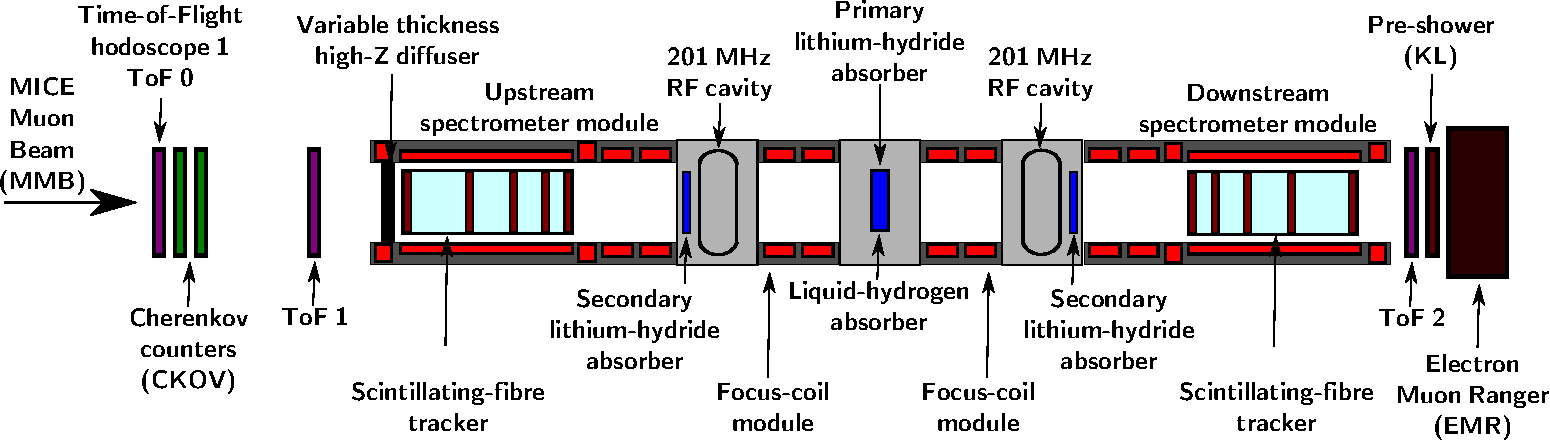
\includegraphics[width=1.0\linewidth]{01-MICE/DEMO_CoolingChannel.pdf}
      \caption{\label{fig:CoolingChannel} The downstream beam line and final cooling channel. The diffuser is used to increase the beam emittance prior to cooling. The primary absorber can be swapped between liquid hydrogen and solid lithium hydride.}
    \end{center}
  \end{figure}

  MICE will represent the first practical demonstration of muon cooling. A schematic of the full MICE cooling channel, including ionisation energy loss and longitudinal accelaration, is shown in figure~\ref{fig:CoolingChannel}.

  MICE is based at Rutherford Appleton Laboratory, U.K., using the ISIS synchrotron as a proton driver to generate the muon beam.  The MICE beamline is described in detail in~\cite{MiceBeamline}.  MICE recently completed Step~I of its programme, consisting of the muon beamline with particle identification (PID). The next step in the programme, Step IV, will introduce the trackers and the first absorber module, producing transverse emittance reduction, and will begin taking data in 2015. The demonstration of sustainable cooling, which includes longitiudinal re-acceleration, will begin data taking in 2017.

%   \begin{figure}[tb]
%     \begin{center}
%       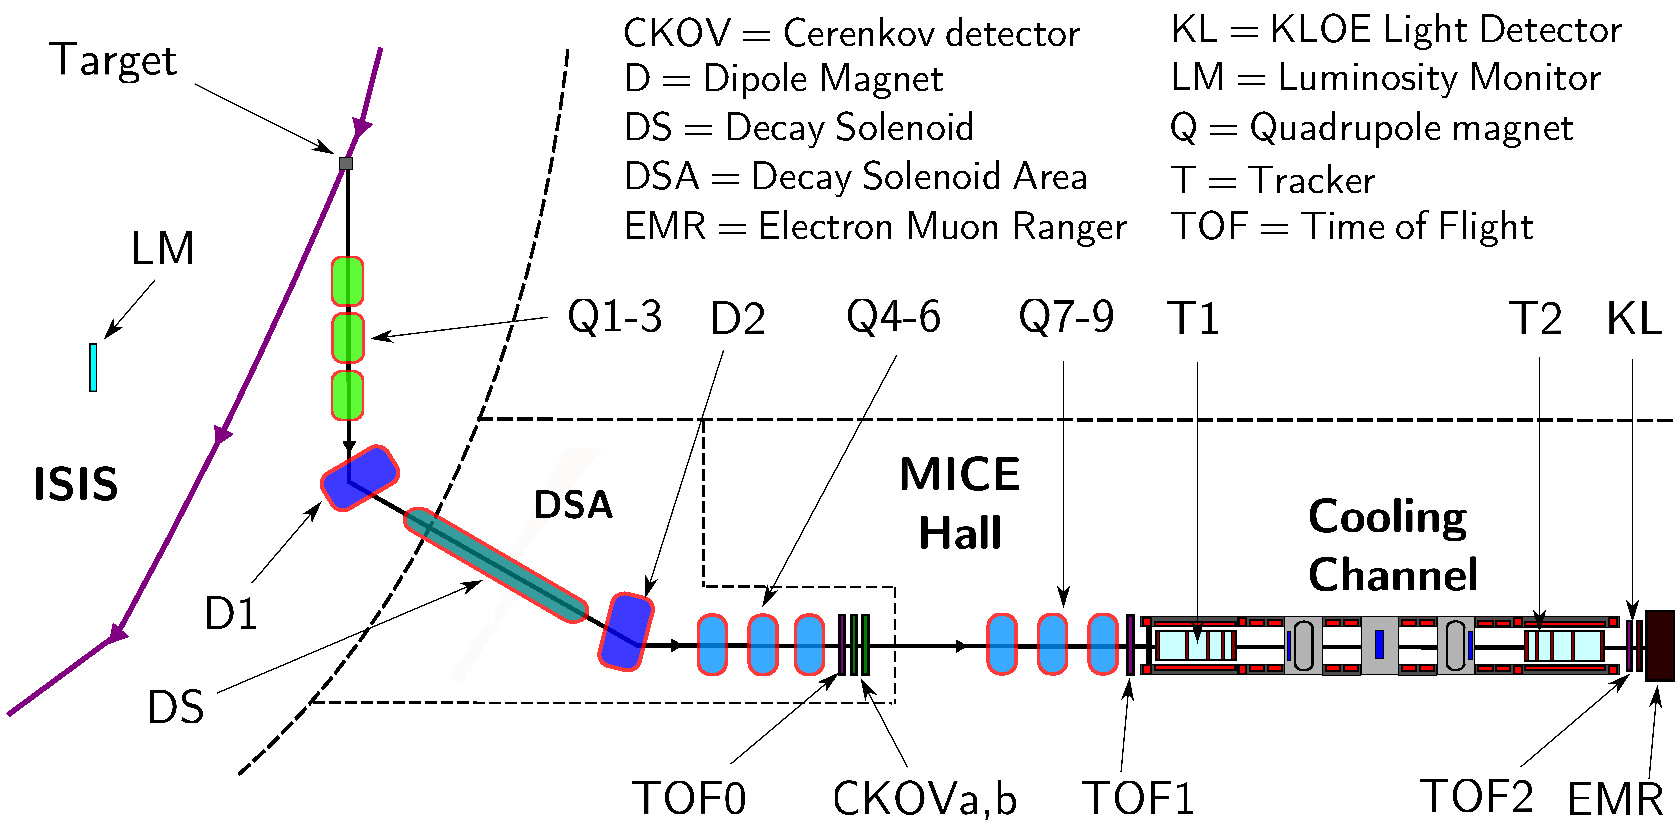
\includegraphics[width=0.75\linewidth]{01-MICE/BeamLineDEMOSans.pdf}
%       \caption{\label{fig:Beamline}The MICE Muon Beamline. A pion production target intercepts the protons of the circulating ISIS beam. Some of the subsequent pions are then captured by quadrupoles and guided down the beamline, passing through various PID dectors along the way, before delivery to the cooling channel itself. Emittance is measured immediately before and after the cooling channel using the scintillating fibre trackers.}
%       \end{center}
%   \end{figure}

  \subsection{The Scintillating Fibre Trackers}
  \label{subsec:Trackers}
  MICE is equipped with two identical, high precision scintillating fibre (``scifi'') trackers, described in~\cite{MiceTrackers}. Each tracker is housed in a superconducting solenoid that provides a uniform 4\,T field over the tracking volume. Tracker~1 is located upstream of the cooling channel, Tracker~2 downstream.  Each tracker consists of 5 detector stations, labelled 1 to 5, as illustrated in figure~\ref{fig:Trackers}. Tracker~1 is orientated such that Station~5 sees the beam first, while Tracker~2 is rotated by 180$^\circ$ such that Station~1 sees the beam first, thus in both trackers Station~1 is always nearest to the cooling channel (see figure~\ref{fig:CoolingChannel}).
  
  \begin{figure}[tbh]
    \centering
    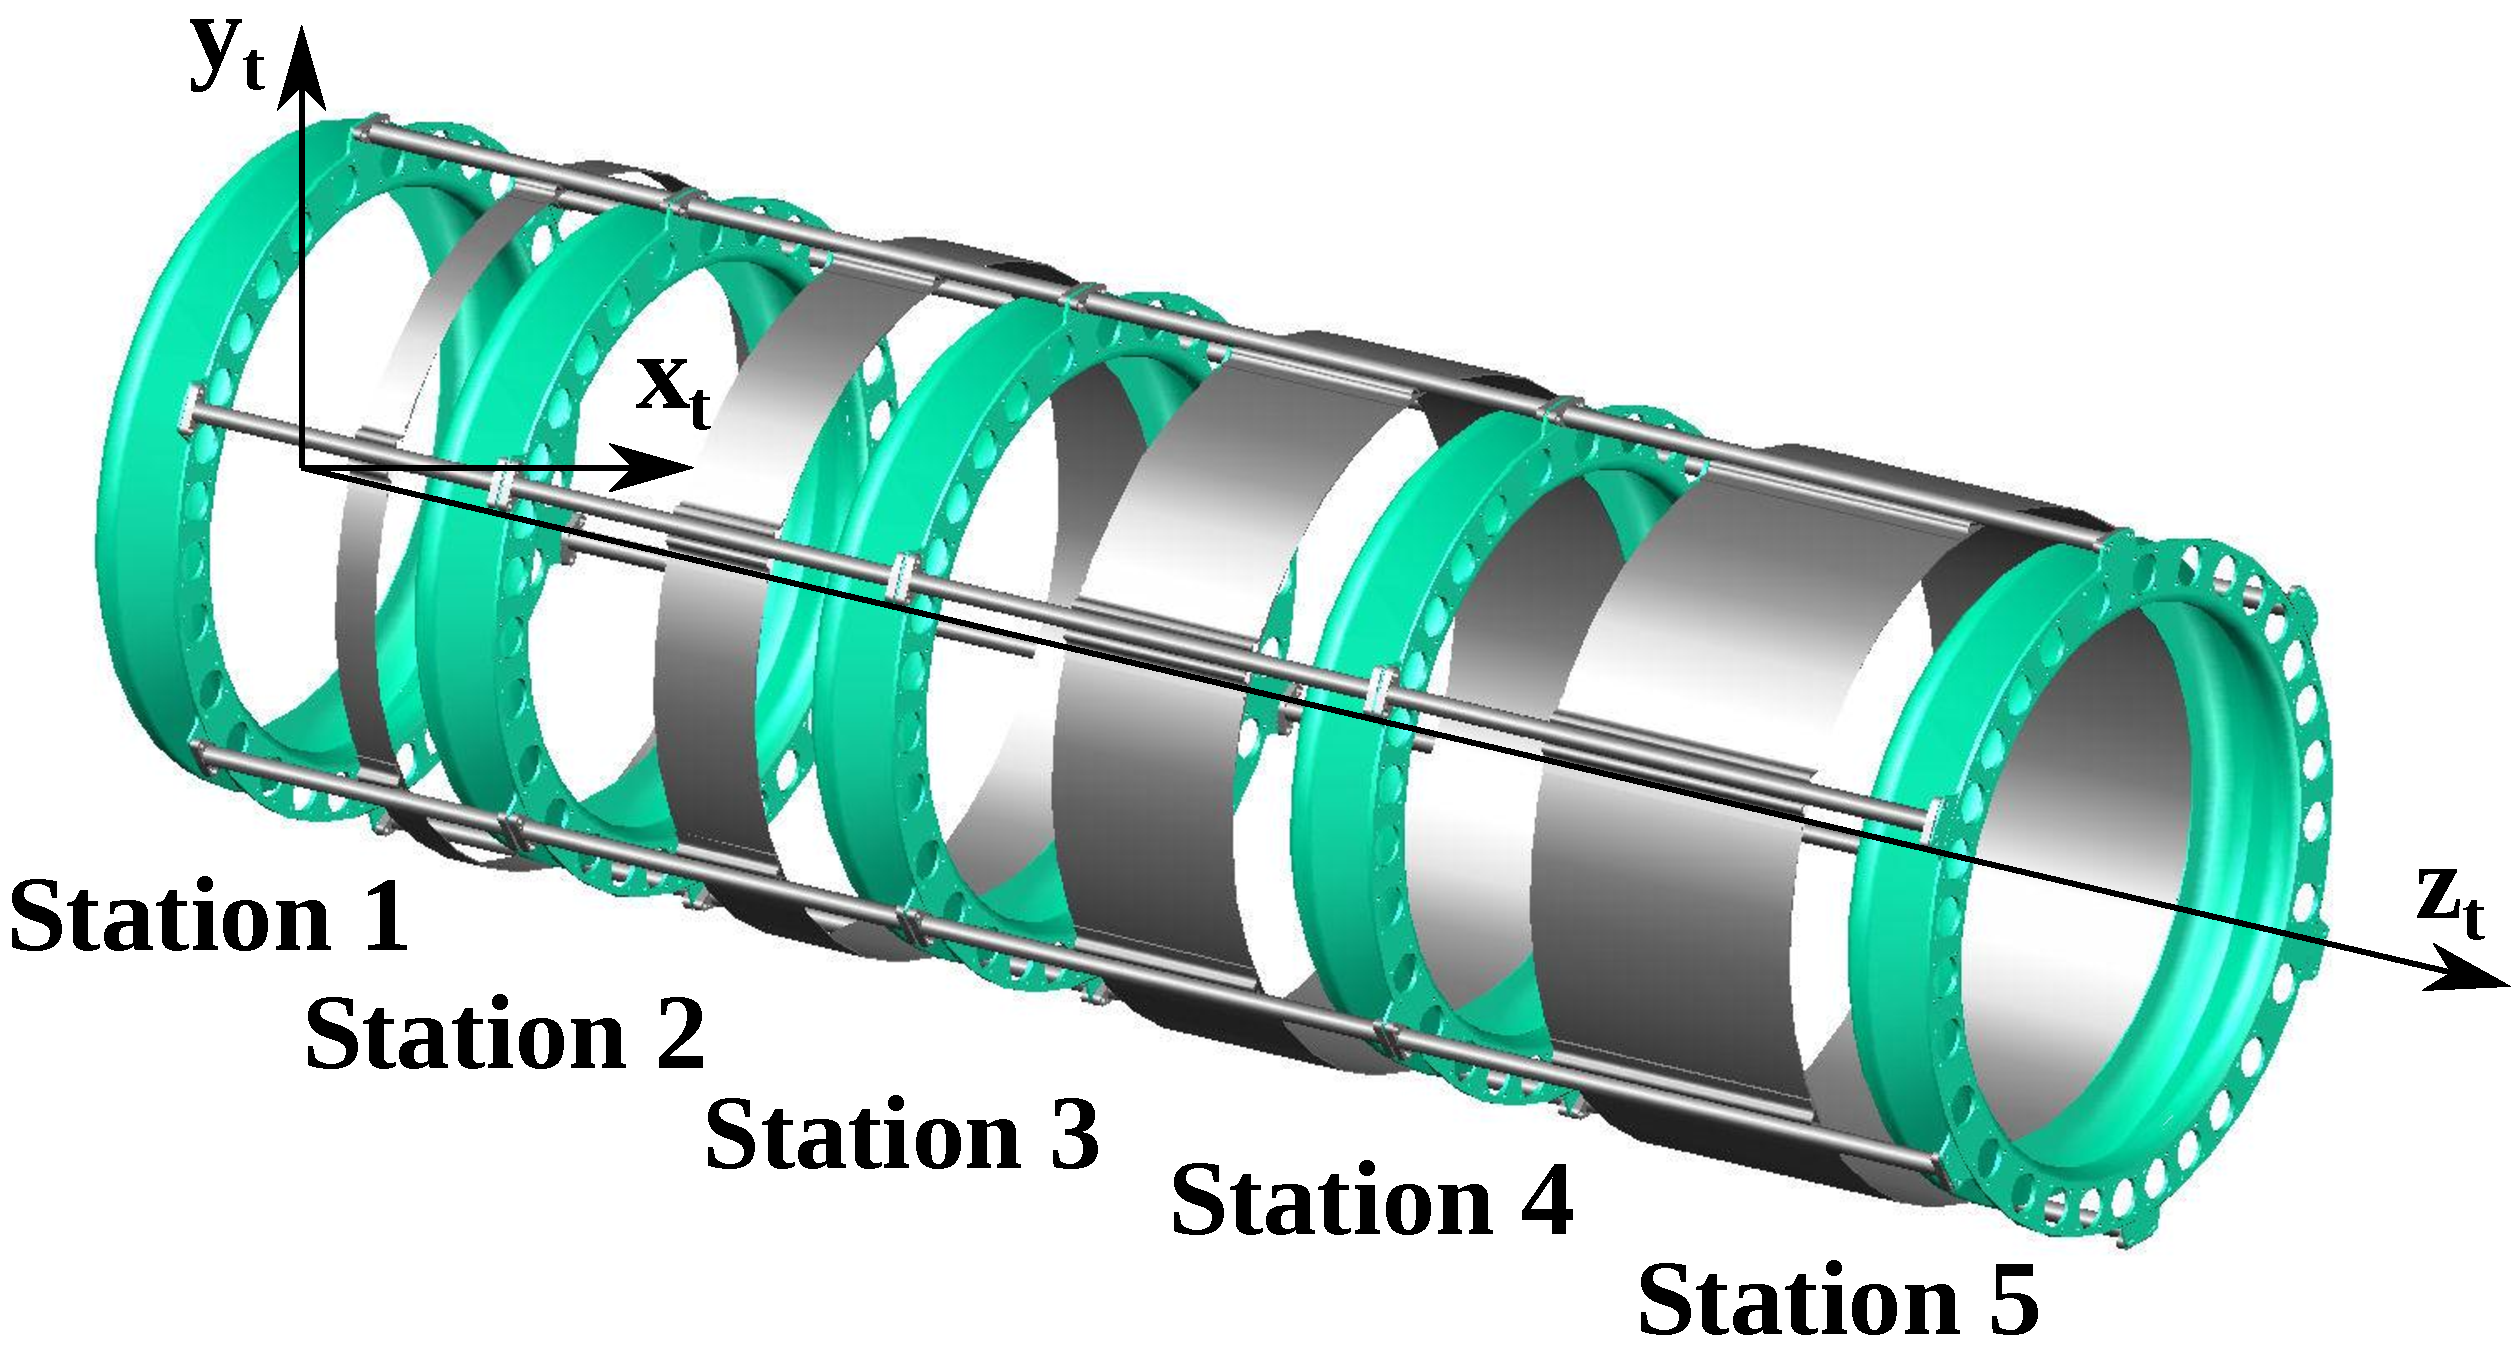
\includegraphics[width=0.5\linewidth]{01-MICE/TrackerFrame.pdf} \hspace{2pc}%
    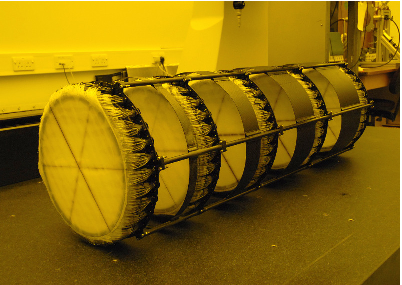
\includegraphics[width=0.35\linewidth]{01-MICE/TrackerPhoto.pdf}
    \caption{\label{fig:Trackers} Left: A schematic of the tracker carbon fibre frame, showing the detector station positions.  The fibre planes are glued on to the upstream edge (smaller $z_t$ position) of the carbon fibre station frames (shown in green). Right: A photograph of a tracker. The orange tint is due to the special lighting needed to protect the fibres. The intersecting lines visible on the station faces indicates the direction of the fibres in each plane.}
  \end{figure}

  Each station is formed of three planes of 350~$\mu$m scintilating fibres, orientated at 120 degrees to each other, attached to a sheet of mylar plastic. The fibres in each plane are arranged in a doublet-layer structure in order to give 100$\%$ coverage of the plane area as illustrated in figure~\ref{fig:DoubletLayer}. A mylar sheet glued to the doublet layer provides mechanical stability. The fibres are collected into groups of seven for readout, each group forming a single channel, as illustrated in figure~\ref{fig:DoubletLayer}b. The planes, also known as views, are labelled $U$, $V$ and $W$. Plane $U$ is attached to the station frame directly, plane $W$ on to plane $U$, and plane $V$ on to plane $W$. The fibre plane orientations are illustrated in figure~\ref{fig:FibrePlaneOrientation}. Each station is oriented such that the fibres in the U plane are vertical. The fibres produce scintillation light when ionising radiation passes through them. Clear-fibre light guides transport the scintillation light to visible light photon counters (VLPCs) in a cryostat for readout (see~\cite{MiceTrackers} for details).

  \begin{figure}[tbh]
    \begin{center}
      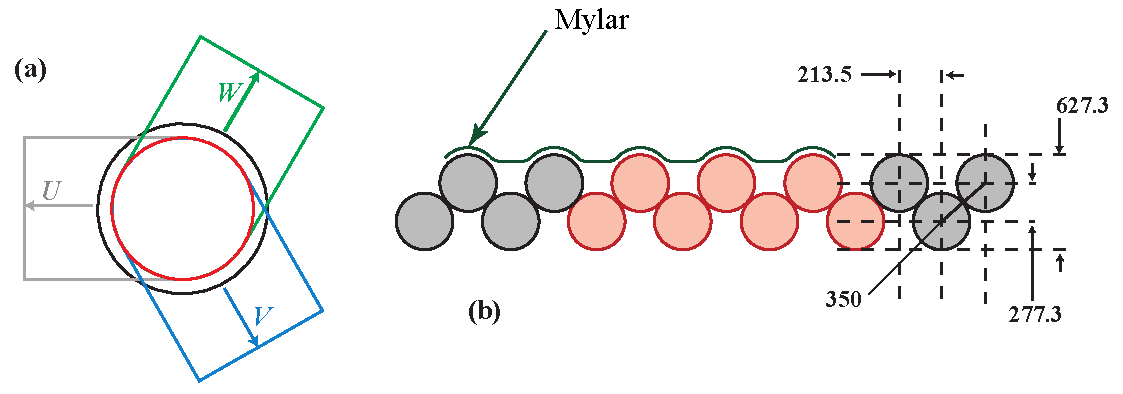
\includegraphics[width=0.85\textwidth]{01-MICE/doublet-layer.pdf}
      \caption{\label{fig:DoubletLayer}(a) Arrangement of the doublet layers in the scintillating-fibre  stations. The outer circle shows the solenoid bore while the inner circle shows the limit of the active area of the tracker. The arrows indicate the direction that the individual 350\,$\mu$m fibres run. (b) Detail of the arrangement of the scintillating fibres in a doublet layer. The fibre spacing and the fibre pitch are indicated on the right-hand end of the figure in \,$\mu$m. The pattern of seven fibres ganged for readout as a single channel, via a single clear-fibre light-guide, is shown in red. The sheet of mylar plastic glued to the doublet layer is indicated. }
    \end{center}
  \end{figure}

  \begin{figure}[tbh]
    \centering
    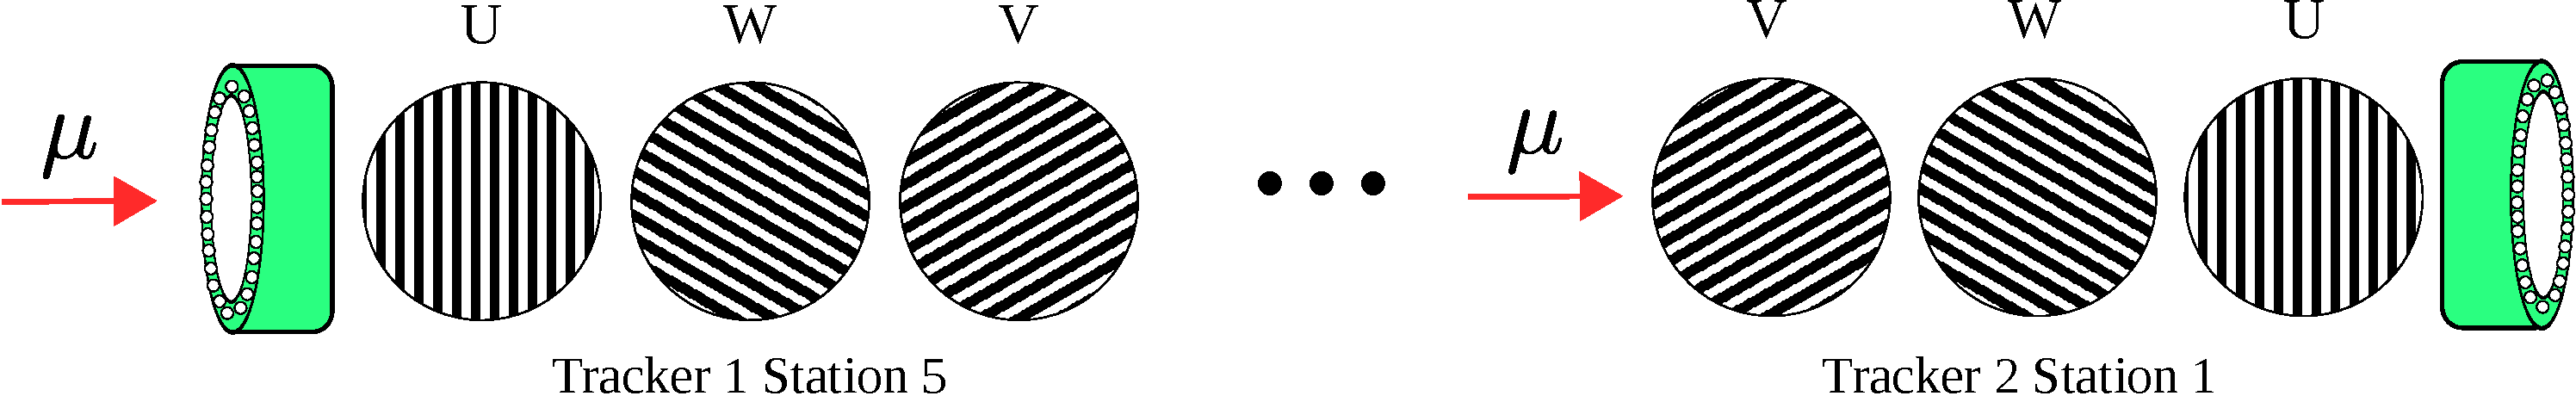
\includegraphics[width=0.95\linewidth]{01-MICE/FibrePlaneOrientation.pdf} \hspace{2pc}%
    \caption{\label{fig:FibrePlaneOrientation} The orientation of the fibres in each plane, as seen be the incoming beam, for both trackers. The green object is station frame. If Tracker~1 was rotated by $180^\circ$ around the centre of the cooling channel, it would be coincident  Tracker~2.}
  \end{figure}
\section{Coordinate systems and Reference Surfaces}
\label{sec:Coordinates}

  \subsection{Channels and Digits}
  The $V$ and $W$ planes each consist of 214 channels, labelled 0 to 213, while the $U$ plane has 212 channels, labelled 0 to 211.  The channel number increases from left to right if a plane is placed mylar side up, with the fibre readout pointing downwards, as illustrated in figure~\ref{fig:DoubletLayerOrder}.

  \subsection{Planes and Clusters}
  The plane reference surface is defined to be the flat plane that is formed by the outer surface of the mylar sheet. The measured position perpendicular to the direction of the fibres in each plane is labelled  $\alpha \in (v, u, w)$, defined to increase in the same direction as the channel number.  The $z$ axis of the plane coordinate system is defined to be perpendicular to the plane reference surface and points in the direction from the mylar sheet towards the fibres. The direction in which the fibres run defines the final plane coordinate, $\beta$, with the direction defined to complete a right-handed coordinate system. The origin of the $(\beta, \alpha)$ coordinate system is taken to be at the centre of the circular active area of the plane.

  \subsection{Stations and Spacepoints}
  The station reference surface is defined to coincide with the reference surface of the $V$ doublet-layer. The station coordinate system is defined such that the $y_s$ axis is coincident with the $v$ axis, the $z_s$ axis is coincident with the $z_p$ axis of the $V$ layer and the $x_s$ axis completes a right-handed coordinate system.
 

  \subsection{Trackers and Tracks}
  The tracker reference surface is defined to coincide with the reference surface of Station~1. The tracker coordinate system is defined such that the $z_t$ axis coincides with the axis of cylindrical symmetry of the tracker as shown in figure~\ref{fig:Trackers}. The tracker $z_t$ coordinate increases from Station~1 to Station~5. The tracker $y_t$ axis is defined to coincide with the $y_s$ axis of Station~1 and the tracker $x_t$ axis completes a right-handed coordinate system. 
  
  \begin{figure}[htb]
    \begin{center}
      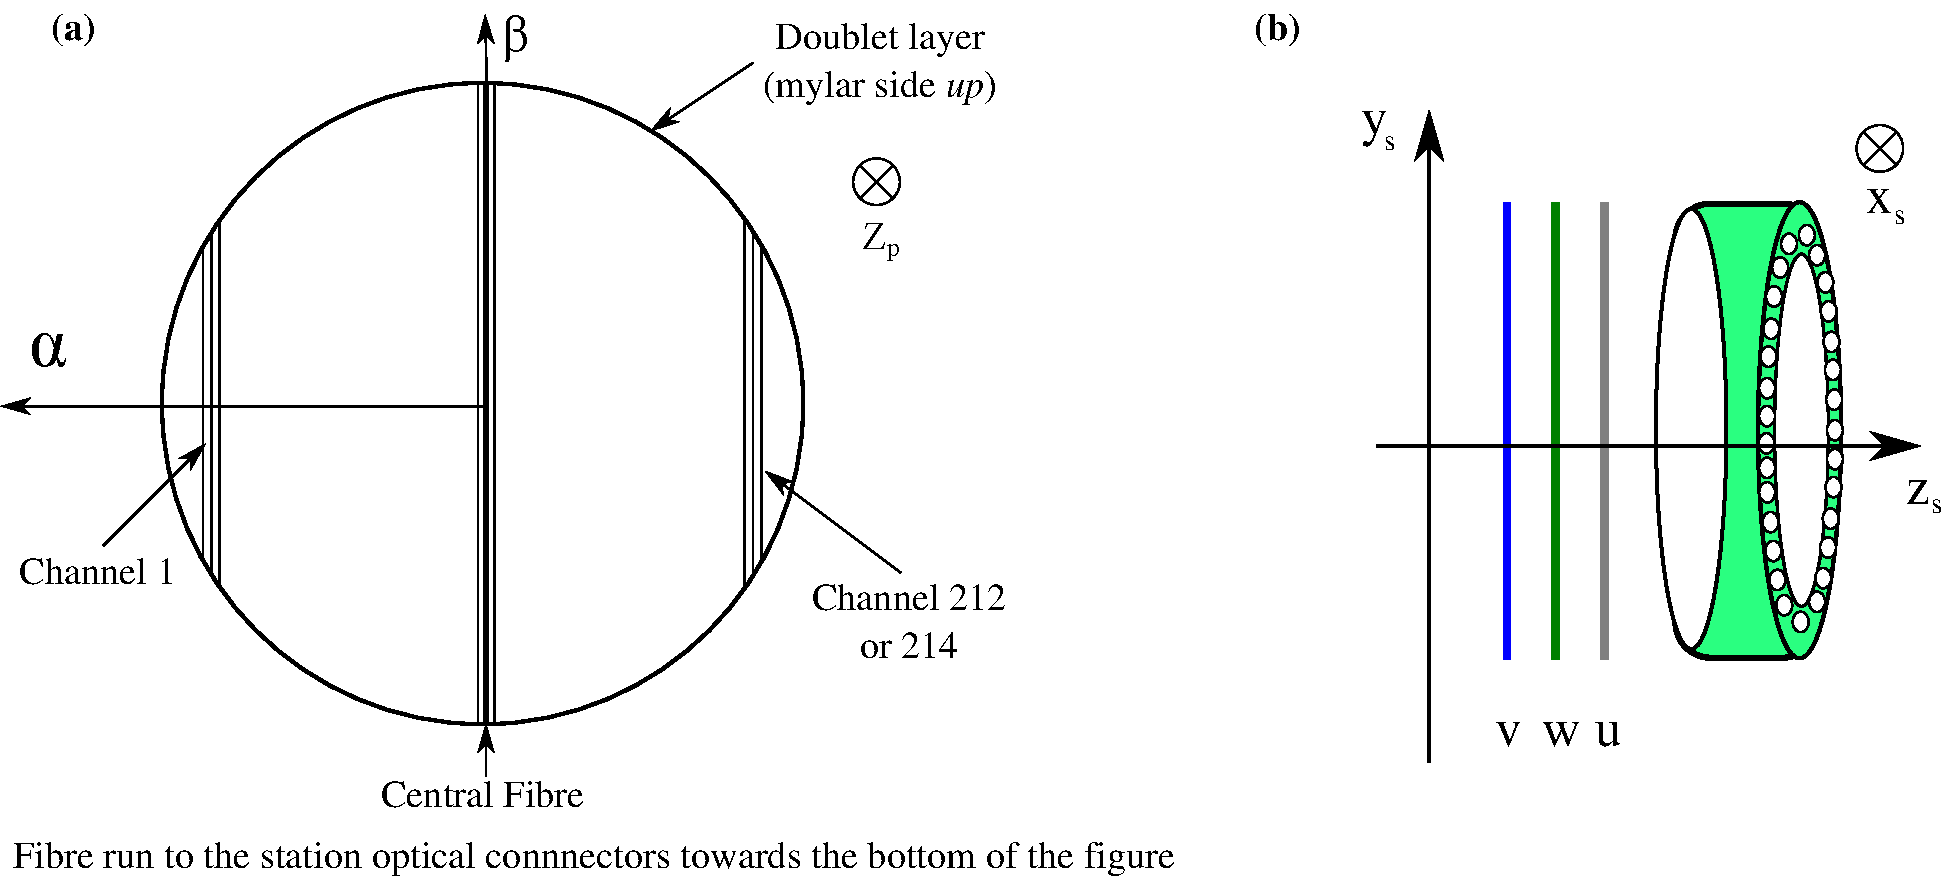
\includegraphics[width=0.9\textwidth]{02-CoordinateSystems/PlaneCoordinatesAndNumbering.pdf}
      \caption{\label{fig:DoubletLayerOrder} (a)~The channel numbering within a plane, and the $(\beta, \alpha, z_p)$ plane coordinate system (a right-handed system).  (b)~The fibre plane ordering with respect to the station body and the station coordinate frame (a right-handed system).  In Tracker~1 the beam approaches from the right, in Tracker~2 from the left. Note that $z_s$ is by definition equivalent to $z_p$ of the $V$ plane.}
    \end{center}
  \end{figure}

\section{The MAUS framework}
\label{sec:MAUS}
The tracker software is part of the MICE software framework, known as MAUS (MICE Analysis User Software)~\cite{MausPaper}. MAUS is used to perform Monte Carlo simulation and both online and offline data reconstruction. It is built using a combination of C++ and Python, with C++ being used for more processor intensive tasks and Python being used more in the code presented to the user.  Simulation is based on GEANT4~\cite{GEANT4}, with analysis based on ROOT~\cite{ROOT}.  ROOT files are used as both the primary input and output data format. MAUS also reads in the custom binary format written by the MICE data acquisition system (DAQ). 

MAUS programmes are defined in a Python script together with a configuration file.  This script allows the user to create programmes by combining different MAUS modules depending on the task at hand, following the Map-Reduce programming model\cite{MapReduce}. The object passed between the modules is known as a ``spill'', representing the data associated with one spill of particles through the MICE beamline (see~\cite{MiceBeamline}).  The modules come in four types: Input; Output; Map; and Reduce.  Input modules provide the initial data to MAUS, from a data file, or from the DAQ. Maps perform most of the simulation and analysis work and may be processed in parallel across multiple nodes.  Reducers are used to display output, such as for online reconstruction plots, and are capable of accumulating data sent from maps over multiple spills, but must be run in a single thread. Output modules provide data persistency.

The tracker software consists four maps and a reducer. The maps cover: digitisation of Monte Carlo data; digitisation of real DAQ data; the addition of noise to Monte Carlo data; and reconstruction. The reducer provides event plots and run information.  %The modules contain little code themselves but instead call C++ classes to perform the work.
\section{Data Structure}
\label{sec:DataStructure}

\subsection{General MAUS, Monte Carlo and DAQ data structures}
\label{subsec:GeneralDataStructure}
A simplified schematic of the tracker data structure, with the relevant entries from the more general MAUS data structure, is shown in figure~\ref{figureDataStructure}.  All the objects listed represent container classes for different parts of the simulation, raw data and reconstruction.  The top level object is known as the spill, which contains the data associated with the burst of particles produced by one dip of the pion production target.  Within the spill the data is split into three branches: real data from the DAQ; Monte Carlo data generated by simulation; and reconstruction data, which is formed from data in either the real or Monte Carlo branches. 

The reconstruction code makes no direct reference to the Monte Carlo information, and has no way to distinguish real from simulated data, thus ensuring that they are treated equally.  The real DAQ data is held in an object known as TrackerDAQ.  This is then further split depending on where the raw data originated; if from the full MICE DAQ then it is stored in a VLSB object or, if the data originated in a cosmic-ray test DAQ, in a VLSB\_C object.

\begin{figure}[bt]
  \begin{center}
    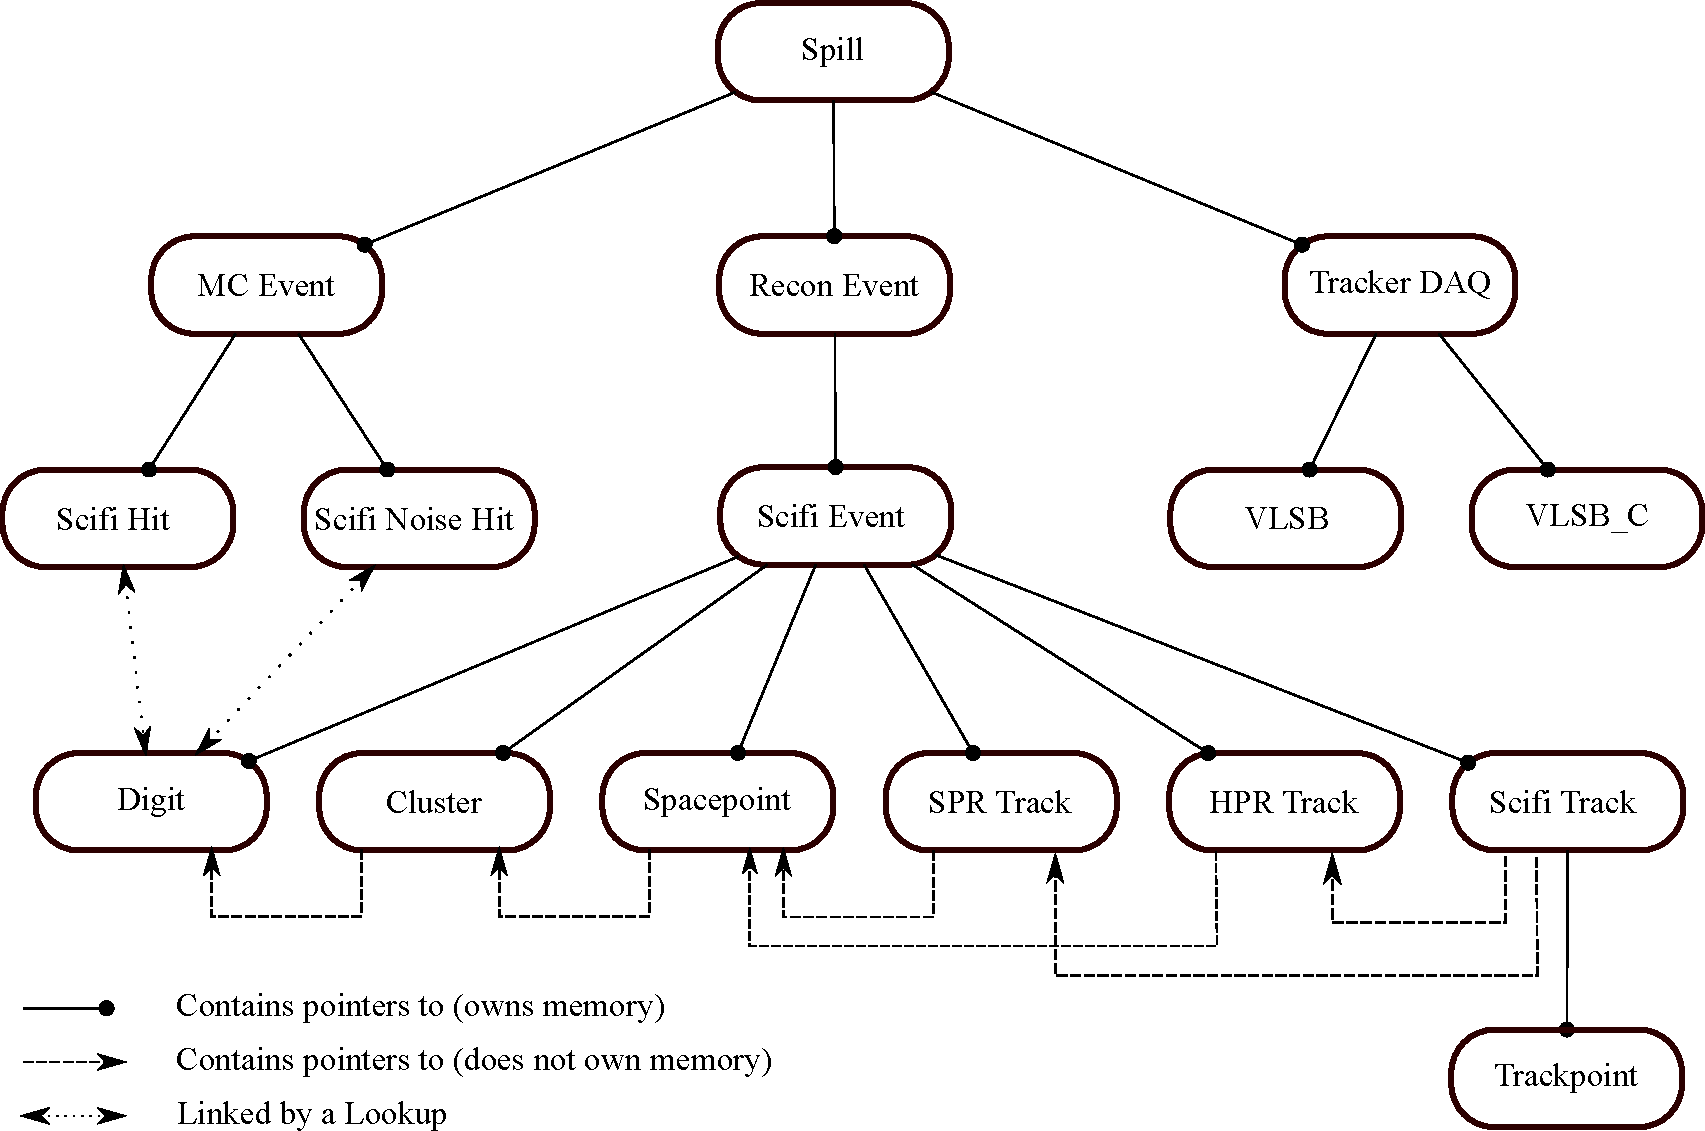
\includegraphics[width=25pc]{04-DataStructure/DataStructureSimple2016.pdf}
    \caption{\label{figureDataStructure}The tracker software data structure, and relevant MAUS data structure.  The spill is the top level object below which data is split into real data, MC data and reconstruction sides. When an object owns the memory of a set of other objects, these are held as standard vectors of pointers. When an object contains cross links to another set of objects, without owning their memory, these are held as a ROOT TRefArray of pointers. SPR = Straight Pattern Recognition, HPR = Helical Pattern Recognition.}
  \end{center}
\end{figure}

The Monte Carlo event holds data on scifi hits produced by tracks passing through sensitive volumes (the fibre planes) and any associated noise hits originating in those planes. The scifi hit is implemented as a class based on the generic Hit class template from which all the different MICE Monte Carlo detector hit classes are derived (see~\cite{MausPaper}).  Other relevant data held in the Monte Carlo event, though not part of the tracker data structure, includes simulated track objects which hold the generated information on position, momentum and particle type.  Such data is used to evaluate the reconstruction performance against the generated data (see section~\ref{sec:Performance}).

\subsection{Tracker reconstruction data structure}
\label{subsec:TrackerReconDataStructure}
The reconstructed data for the tracker is held in the SciFiEvent class.  This contains C++ standard library vectors of the following container classes that represent the higher level reconstructed tracker data:
\begin{itemize}
  \item ``SciFiDigits'' represent the digitisation of a detector channel response to an incident track;
  \item ``SciFiClusters'' represent groups of neighbouring Digits arising from the same particle crossing multiple channels;
  \item ``SciFiSpacepoints'' group Clusters from adjacent detector planes to give a real space position in terms of $(x, y, z)$;
  \item ``SciFiStraightPRTracks'' group together Spacepoints from different tracker stations when the originating track is straight (i.e. when the enclosing field is off). %The track parameters given in eqn.~\ref{eqn:StraightTrackParameters} are also stored;
  \item ``SciFiHelicalPRTracks'' group together Spacepoints from different tracker stations when the originating track is helical (i.e. when the enclosing field is on). %The track parameters given in eqn.~\ref{eqn:HelicalTrackParameters} are also stored;
  \item ``SciFiTracks'' hold the final Kalman fit parameters of the particle track. SciFiTracks also contain SciFiTrackPoints, which hold the fit parameters at each detector plane, including the momentum and position of the track.
\end{itemize}

\subsection{Cross links and the Monte Carlo - Reconstruction bridge}
\label{subsec:CrossLinksAndMCBridge}
Each higher level object also contains cross links in the form of pointers back to the objects within the SciFiEvent which were used to create it; thus Clusters contain pointers to Digits, Spacepoints to Clusters, Pattern Recognition Tracks to Spacepoints, and SciFiTracks to Pattern Recognition Tracks. In this manner all higher level objects can be traced back fully to the original Digits.  

In the case of a Monte Carlo run the Digits themselves are linked via an ID number and lookup table back to the Monte Carlo hits used to produce them. The ID is defined as \textit{tspccc}, where \textit{t} is the tracker number, \textit{s} is the station number, \textit{p} is the plane number, and \textit{c} is the channel number.  This structure means the reconstruction branch has no direct reference to the Monte Carlo data.
\section{Geometry}
\label{sec:Geometry}

  The absolute position of each tracker station was determined by use of a coordinate measuring machine (CMM) at Imperial College London~\cite{MiceTrackers}.  The measurements were made by supporting the trackers upon blocks on the CMM. The tracker was not fixed to the supports to avoid introducing extra stresses which might distort the frame. The position of the stations was then determined with respect to station 5. (see table~\ref{tab:CMM}).
  
  \begin{table} [tbp]
  \begin{center}
  \begin{tabular} {|c|c|c|c|c|c|}
    \hline
    \multicolumn{6}{|l|}{Tracker 1 offsets in mm} \\
    \hline
    & Station 1 & Station 2 & Station 3 & Station 4 & Station 5 \\
    \hline
    X & 0.0 & -0.5709 & -1.2021 & -0.5694 & 0.0 \\
    Y & 0.0 & -0.7375 & -0.1657 & -0.6040 & 0.0 \\
    Z & -1099.7578 & -899.7932 & -649.9302 & -349.9298 & 0.0 \\
    \hline
    \hline
    \multicolumn{6}{|l|}{Tracker 2 offsets in mm} \\
    \hline
    & Station 1 & Station 2 & Station 3 & Station 4 & Station 5 \\
    \hline
    X & 0.0 & -0.4698 & -0.6717 & 0.1722 & 0.0 \\
    Y & 0.0 & 0.0052 & -0.1759 & -0.2912 & 0.0 \\
    Z & -1099.9026 & -899.009 & -650.0036 & -350.0742 & 0.0 \\
    \hline
  \end{tabular}
  \caption{\label{tab:CMM} Position of tracker stations from CMM measurements, positions taken with respect to reference surface.}
  \end{center}
  \end{table}
  
  Tracker station positions are stored in the MICE configuration database (CDB). The CDB is a bi-temporal database, alterations are tracked by date and run number, ensuring the proper geometry is used in analysis of historic data.  Configurations are stored in the CDB as a collection of XML files which are translated into the native MAUS format "MICE modules", at run-time.  The MICE modules are text documents and contain all the information needed to simulate the various MICE systems and detectors. The rotation convention adopted in all the MAUS geometry is that of interpreting rotations as passive rotations of the coordinate axis, as opposed to active rotations of the geometry elements. This is done in order to stay consistent with GEANT4.
  
  MAUS uses the same detector geometry descriptions for both Monte Carlo and real data and may be called on by the reconstruction as needed.  The only differences between the Monte Carlo and the real geometries relate to non-active portions of the experiment and field mapping. In particular, only the Monte Carlo geometry contains the epoxy resin, which was used in securing the individual scintillating fibres to the tracker station body, and the mylar sheets to support each doublet-layer. The carbon fibre body of the trackers have not been included in either the real or Monte Carlo geometries as their effect on the beam is expected to be minimal. The active volume of each tracker is given by a cylinder of 150~mm radius, which is used to define the fiducial volume for the reconstruction.
  
  Alignment of the individual tracking stations and the trackers themselves to the solenoid axis will be completed using data taken during commissioning.
  
  
\section{Simulation}
\label{sec:Simulation}

The simulation of the MICE trackers is designed as a module for the MAUS software framework.  The simulation makes use of the GEANT4 standard physics libraries to describe a particle motion's through the scintillating fibre material and uses various statistical models in describing the effects of electronic noise.  The trackers are simulated on a per fibre basis and layered into the fibre planes in the expected doublet layer as shown in figure~\ref{fig:DoubletLayer}. 

The MAUS framework invokes a beamline module to generate a simulated beam, according to pre-defined user parameters.  A particle incident upon a tracker fibre is stepped through, in accordance with the defined parameters. GEANT4 is invoked in each of these steps in determining the resulting momentum change of the particle and the magnitude of energy  deposited into the fibre.  These values are recorded individually, the current step used in determining where the next step is taken, and recorded before the next step is processed.  After a defined number of particles have been generated and stepped through the experiment the results are collected into a MICE spill and sent to the tracker MC module for processing.  

Each one of the incoming MC hits has a simple conversion factor applied which determines the raw number of photo electrons (NPE) generated.  A single interaction with a scintillating fibre is simulated by many steps through the material and the figure for any one step is not limited to integer values.  The raw NPE from every step through the fibre is summed and feed into the simulation of noise in the tracker electronics (see section \ref{subsec:Noise}).

The final result from this process, which includes the channel number, the final processed NPE, and timing information from GEANT4 are used to create a SciFiDigit.  This final result is as described in section~\ref{subsec:GeneralDataStructure}, and the output Digit from the MC is identical to that created from DAQ data.  After all hits have been processed the data is handed back to MAUS to be processed by the tracker reconstruction modules.

  \subsection{Noise}
  \label{subsec:Noise}
  The MC noise simulation consist of two modules, false signal due to thermally excited electrons within the VLPC cassettes and a smearing due to random noise in the tracker electronics.  This is in addition to noise introduced by particle decays handled outside of the tracker MC by the GEANT4 simulation.
  
  Simulation of the thermally excited electrons is performed before the smearing simulation.  The dark count is an uncorrelated process that is selected to occur with a magnitude of 1.0 PE in 1.5$\%$ of a data taking window.  Actual rate is determined by the setting of the voltage bias in the VLPC cassettes which as a direct effect on the final signal size.  The process is described as a Poisson distribution.  Studies are under way to understand this effect in each cassette. 
  
  The results from the GEANT4 physics simulation and the Poisson dark count simulation are combined and smeared to determine the final NPE signal.  The signal from the GEANT4 simulation can take any value, however, it is unreasonable to expect anything other than an integer number of photons, as such this incoming signal is changed to its nearest integer value. The value is smeared as described by a Gaussian with a sigma derived from a study of carried out in May 2012 of a single station in beam.
  
  The smeared result is then fed through a process that simulates the effects of the analogue to digital converters (ADCs).  This process serves to chop the information up into bins of $2^8$ discreet values.  The exact values of these bins is determined from the tracker calibrations and varies with the with the channel placement into the electronics.  Overflows are equivalent to the maximum signal.  
\section{Reconstruction}
\label{sec:Reconstruction}
The reconstruction process is illustrated in figure~\ref{fig:DataFlow} for both real and simulated data.

\begin{figure}[tbh]
  \begin{center}
    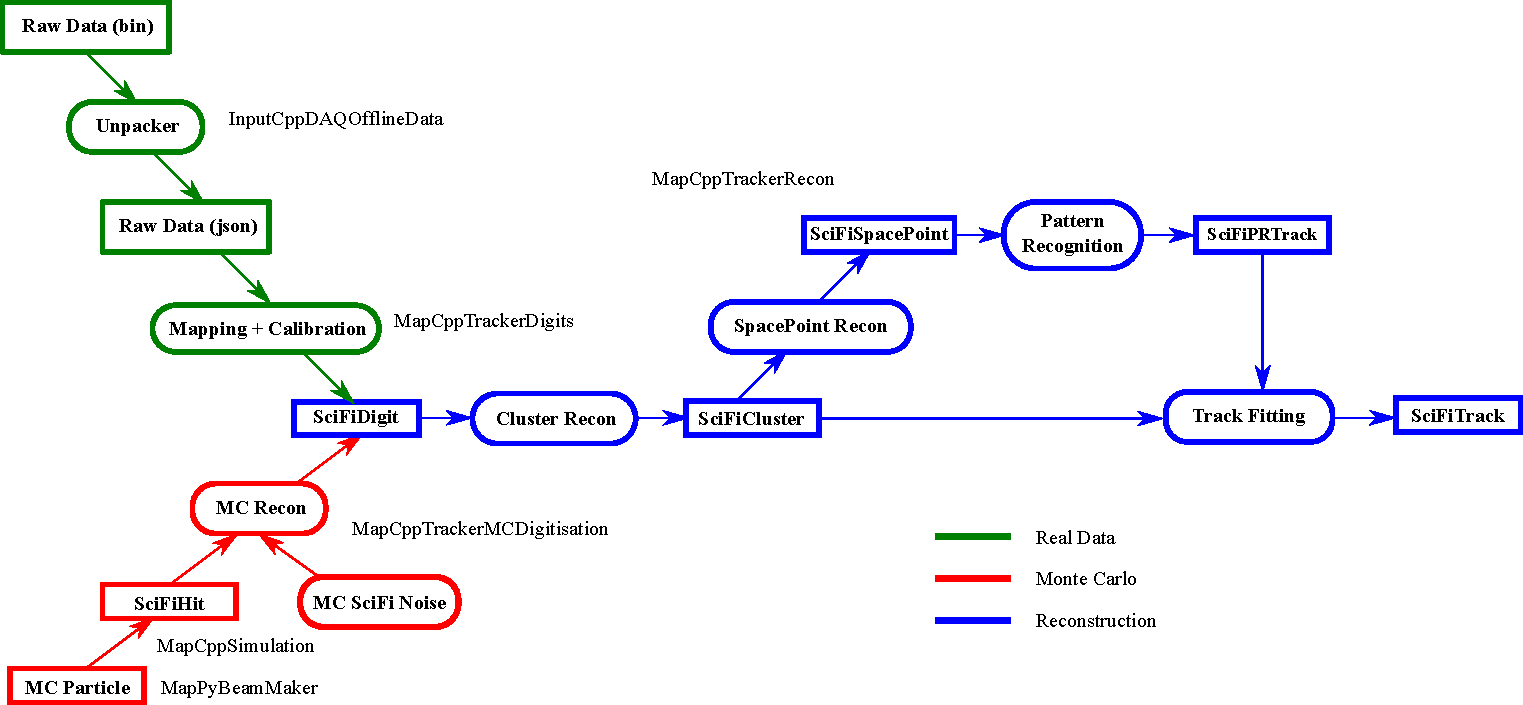
\includegraphics[width=0.95\linewidth]{07-Reconstruction/DataFlow2014.pdf}
    \caption{\label{fig:DataFlow} The reconstruction data flow. Data originates either from simulated or real data, the two branches meet after Digitisation, after which the reconstruction proceeds identically for both.  The relevant MAUS modules for each step are indicated.}
  \end{center}
\end{figure}

  \subsection{Digitization}
  \label{subsec:Digitization}
  For real data the electronic signals produced by the VLPCs are Digitised using analogue-to-Digital converters (ADCs). The DAQ system records the pulse height for each DAQ channel.  Channel-by-channel cailbration constants are used to convert the ADC value to a signal in units of photo-electrons (PE) and the VLPC channel number to tracker channel number.  This information is then used to form a Digit.  The analagous process for Monte Carlo data is described in section~\ref{sec:Simulation}.

  \subsection{Clustering}
  \label{subsec:Clustering}
  A particle that traverses a plane will generate a hit in one or at most two adjacent channels.  An isolated hit or hits in two adjacent channels form a Cluster.  
  
  The Clustering algorithm loops over every combination of pairs of Digits in a SciFiEvent and combines any that occur in neighbouring channels in the same plane. In the case of multi-Digit Cluster, the average channel value is used. The Cluster positioning is defined by the coordinates $(\alpha, \beta)$ where $\alpha$ and the direction of $\beta$ have been defined in Section ~\ref{subsec:PlaneAndClusters}. In the case of two overlapping active channels the value for $\beta$ is determined by solving:
  
  \begin{equation}
    \begin{pmatrix}
     \alpha_1 \\ \beta_1
    \end{pmatrix} = R_{1}^{-1} R_2
    \begin{pmatrix}
      \alpha_2 \\ \beta_2
    \end{pmatrix}
  \end{equation}
  
  \noindent
  where $R_1$, $R_2$ are the rotation matrices that correspond to the orientation of the specified plane. 

  \subsection{Spacepoint Reconstruction}
  \label{subsec:SpacepointReconstruction}
  For each station the constituent planes are searched for Clusters which can be used to define a Spacepoint. Spacepoints are defined by Clusters from all three planes (a triplet Spacepoint) or for any two out of the three planes (a doublet Spacepoint). 
  From the Cluster coordinates, $(\alpha, \beta)$, the $(x, y)$ coordinates of the Spacepoint are determined by rotating into tracker frame.

  \subsubsection{Cluster selection}
  \label{subsubsec:ClusterSelection}
  In order to determine which Clusters from each plane originate from the same track we follow Kuno's conjecture\cite{MiceTrackers} which states that, for a given triplet Spacepoint, the sum of the channel numbers of each Cluster will be a constant.  So if $n^u$, $n^v$ and $n^w$ are the fibre numbers of the Clusters in $u$, $v$ and $w$ and $n^u_0$, $n^v_0$ and $n^w_0$ are the corresponding central channel numbers. Three Clusters form a space point  if:
  \begin{equation}
    | (n^u + n^v + n^w) - (n^u_0 + n^v_0 + n^w_0) | < K \, .
  \end{equation}
  where $K$ is a constant, take by default as 3.0.
  
  Once all triplet Spacepoints have been found, doublet Spacepoints are created from pairs of remaining Clusters. 

  % \subsubsection{Crossing Point Calculation}
  % \label{subsubsec:CrossingPointCalculation}

  \subsection{Pattern Recognition}
  \label{subsec:PatternRecognition}

  Pattern recognition is based on looping over different combinations of Spacepoints and performing a fit using a simple linear least squares technique.  The algorithm treats helical and straight tracks separately, though much of the code is shared. Helical track finding is attempted first then, once all possible helical tracks have been found, any remaining unmatched Spacepoints in the SciFiEvent are passed to the straight line fitting rountines.

   \subsubsection{Helical Pattern Recognition}
   \label{subsubsec:HelicalPatternRecognition}

   The helical pattern recognition is performed in cylindrical co-ordinates $(r, \phi, z)$ where the turning angle $\phi$ defined for $0 \rightarrow \infty$ is distinguished from $\phi '$ the reduced turing angle defined  for $0 \rightarrow 2\pi$. For the helix $s$ is the distance the particle travels measured along the helix. The helix is described by: the circle it describes in the transverse plane $(x_{centre}, y_{centre}, radius)$; $s_0$ the value of $s$ where the helix crosses the reference plane; and $t_s = ds/dz$, which describes the tightness of the coiling. $\phi_0$, the angle of the track as it crosses the tracker reference plane, equivalent to $s_0$, is also used. 

   To find a track one Spacepoint is selected from each station and a circle is fitted in the $(r, \phi')$ projection. If the $\chi^2$ of this fit is sufficiently small (by default less than 15.0 multiplied by the number of degrees of freedom) then the value of $\phi$ is used to generate $s$ and a straight line fit is performed in the $(z,s)$ plane, and if the $\chi^2$ in this projection is also small (by default less than 4.0 multiplied by the number of degrees of freedom) the track is accepted.  $\phi$ itself is determined from $\phi'$ by exploiting the different distances in $z$ between successive tracker stations.  The change in $\phi$ between the hits in any two stations, divided by the distance between those stations, gives a constant which is the same for any pair of hits.  This can then be used to infer the true values of $\phi$.

   All possible combinations of five Spacepoints, one from each station are tested. Points can only be associated with one track. Then all combinations of any remaining Spacepoints are searched, this time requiring Spacepoints from four out of the five stations to form a helix. Tracks with momentum almost parallel to the solenoid axis (i.e. with low transverse momentum, $p_T$) will not suffer an appreciable bend and will not be found by the helix search and so any Spacepoints remaining after the helical tracks have been found are passed to the straight track finding algorithm.

    \subsubsection{Straight Line Pattern Recognition}
    \label{subsubsec:StraightLinePatternRecognition}

    Straight lines are fitted to the Spacepoints when there is no magnetic field and on any Spacepoints remaining after the helix fit is complete. The latter is to identify tracks with a small $p_T$ which are not bent sufficiently in the magnetic field to form a recognisable helix (it has been observed from Monte Carlo studies that the efficiency of the helix finding algorithm begins to tail off for tracks with $p_T < 10 MeV/c$).

    The fit is done in Cartesian coordinates and the track parameters are: $(x_0, y_0, t_x, t_y)$ where $t_x = dx/dz$ and $t_y = dy/dz$. Two Spacepoints are chosen in the outer chambers and a road is created between them. Any Spacepoints in the road are fitted, using Least Sqaures, in the $(x,z)$ and $(y,z)$ planes. The Spacepoints with the lowest $\chi^2$ are chosen as long as their value is less than a predefined cut value (by default less than 15.0 multiplied by the number of degrees of freedom). As in the helical case, following the completion of the full 5 point track search, tracks with Spacepoints in 4 out of the 5 stations are searched for. For the straight case only, following the completetion of the search for 4 point tracks, a search is also made for tracks with Spacepoints in only 3 out of the 5 stations. 

   \subsection{Track Fit}
   \label{subsec:FinalTrackFit}
   The final track fit was implemented using a track-orientated Kalman filter\cite{Fruhwirth,Billoir}, which can be shown to be an optimal linear fitter, that takes into account all correlations and measurements, for a linear system. The Kalman Filter is an iterative algorithm that incrementally propagates an estimate of the current track state between measurement planes, using measurement information to ``filter'' the state, improving the estimate of the track state.
   
   For the helical track fit, the system is only approximately linear, hence an extended Kalman filter was implemented which analytically propagates the track states between measurements, while the covariance matrices are propagated using a first-order linear approximation to the non-linear system.

   Pattern recognition provides a set of Clusters that are associated with a track, which passed the selection criteria, and a parameterisation of that track based on a least squares fit to the points by a helix or a straight line as appropriate. The track parameters calculated from the least squares fit are used to provide the seed for the Kalman fit and the raw Cluster information is used as the measurement data. The flexibility of the Kalman algorithm permits the effects of individual planes (multiple coulomb scattering (MCS) and energy loss), in addition to the material effects of the Helium gas within the tracker, to be accounted for between each measurement point.

     \subsubsection{Kalman Filtering}

     The track is modelled as a discrete state space function of $z$ (the direction of the beam), indicated by the subscript, $k$, where each tracker plane corresponds to a trackpoint and contains a measurement and a track state. Equation~\ref{equ:kalman_system_equation} describes how the true state space vector, $\mathbf{x}_{k,t}$, is assumed to propagate to a subsequent measurement plane. The matrix, $\mathbf{F}_k$, is the Kalman Propagator and describes the first order description of the propagtion between measurement planes. $\mathbf{w}_k$ represents some ``process noise'', which may affect the system between the two measurement planes and is assumed to be gaussian distributed white noise.
    \begin{equation}
      \mathbf{x}_{k,t} = \mathbf{F}_{k-1}\mathbf{x}_{k-1,t} + \mathbf{w}_{k-1}
      \label{equ:kalman_system_equation}
    \end{equation}
    \begin{equation*}
      \textrm{exp}(\mathbf{w}) = 0 \quad\quad \textrm{and} \quad\quad \textrm{cov}(\mathbf{w}) = \mathbf{Q}
    \end{equation*}
     
     The tracker measurements are interpreted in a different state space to the track, allowing measurements of any dimension to be used to filter the track. Equation~\ref{equ:kalman_measurement_equation} describes how the true track state is ``measured'' to be transformed into the measurement space. The matrix, $\mathbf{H}_k$, is the Kalman Measurement Matrix and describes, to first order, the transformation from track state space to the measurement state space. $\mathbf{\varepsilon}_k$ represents some ``measurement noise'' which may smear the measurement of the true state space, it is also assumed to be gaussian distributed.
    \begin{equation}
      \mathbf{m}_k = \mathbf{H}_kx_{k,t} + \mathbf{\varepsilon}_k
      \label{equ:kalman_measurement_equation}
    \end{equation}
    \begin{equation*}
      \textrm{exp}(\mathbf{\varepsilon}) = 0 \quad\quad \textrm{and} \quad\quad \textrm{cov}(\mathbf{\varepsilon}) = \mathbf{V}
    \end{equation*}

    For each measurement plane that contains a measurement, the current estimate for the track state vector is ``filtered'' using the measurement information. This is acheived using the residual between the estimate for the track state and the measurement data, in the measurement state space. Equation~\ref{equ:kalman_state_filtered} describes how the predicted state vector, $\mathbf{x}_{k}^{k-1}$ is filtered using the Kalman Gain Matrix, $\mathbf{K}_k$, to produce the filtered track estimate, $\mathbf{x}_k$. Equation~\ref{equ:kalman_gain_matrix} defines the Kalman Gain Matrix.
    \begin{equation}
      \mathbf{x}_k = \mathbf{x}_k^{k-1} + \mathbf{K}_k ( \mathbf{m}_k - \mathbf{H}_k \mathbf{x}_k^{k-1} )
      \label{equ:kalman_state_filtered}
    \end{equation}
    The predicted covariance matrix, $\mathbf{C}_k^{k-1}$, is filtered in a similar  fashion to produce the filtered covariance matrix, $\mathbf{C}_k^{k}$, as described in equation~\ref{equ:kalman_covariance_filtered}:
    \begin{equation}
      \mathbf{C}_k = ( \mathbf{I} - \mathbf{K}_k \mathbf{H}_k ) \mathbf{C}_k^{k-1}
      \label{equ:kalman_covariance_filtered}
    \end{equation}
    The Kalman Gain matrix is calculated by:
    \begin{equation}
      \mathbf{K}_k = \mathbf{C}_k^{k-1} \mathbf{H}_k^\mathsf{T} (\mathbf{V}_k + \mathbf{H}_k \mathbf{C}_k^{k-1} \mathbf{H}_k^\mathsf{T})^{-1}
      \label{equ:kalman_gain_matrix}
    \end{equation}

    The sequence of prediction and filtering is repeated for all the measurement planes, starting from station~5, plane~2, where the predicted state vector and covariance matrix is determined from the pattern recognition fit parameters, to station~1, plane~0, the reference plane. Once the reference plane has been reached, the state vector will have been sequentially filtered using all the measurements in turn to create the optimal estimate of the track state at that plane. The fit can then be smoothed, whereby the optimal state vector is propagated in reverse down the length of the track, such that all the subsequent measurements can be used to re-adjust previous state vector estimates. This is dsecribed in~\cite{Fruhwirth}


    \subsubsection{The MAUS Kalman Filter Implementation}
    In order to implement a flexible re-usable Kalman Filter, the core algorithm was implemented without any dependencies on phase space dimensions or physical effects. Due to this only the system specific functionality need be provided for a complete implmentation.
    The principal components of the implementation are: propagation routines for both helical and straight tracks; a measurement routine that correctly transforms the track state space into the measurement state space; and approximations for the process and measurement noise.
    
    The measurements correspond to individual Clusters, hence the parameter $\alpha$ (see section~\ref{subsec:PlaneAndClusters}) forms a one-dimensional measurement state. The measurement noise corresponds to the statistical spread of measurements within a single channel in the tracker readout. If the channel is modelled as a top-hat function, the variance of the function is calculated as $w^2/12$, where $w$ corresponds to the width of the channel. Therefore the measurement noise was assumed to be $w/\sqrt{12}$ for all Clusters.

    The process noise was implmented as a combination of MCS and energy straggling. The mean energy loss was is calculated using the Bethe-Bloch equation and applied during the propagation stage. The noise term itself is calculated per increment, as an RMS scattering angle using an implementation of the Highland formula (equation~\ref{equ:highland_formula}), in a fashion almost identicle to the GEANT4 implementation:
    \begin{equation}
      \theta_{RMS} = \frac{13.6\textrm{MeV/c}}{\beta c p} z \frac{x}{X_0}\left( 1 + 0.038 \ln(\frac{x}{X_0} \right)
      \label{equ:highland_formula}
    \end{equation}
    where $\theta_{RMS}$ is the RMS scattering angle through a finite length of material, $\beta c$, $p$ and $z$ are the velocity, momentum and charge of the particle in question, and $x/X_0$ represents the total path length through the material per radiation length. Although the RMS scattering angle does not form a gaussian distribution, the first order approximation is believed to be sufficient.

%    \subsubsection{Goodness of fit}
%    For each fitted track, a test statistic is computed, which is the $\chi^2$ sum over all the trackpoints. It is calculated by $\chi^2\sum_{k=0}^{k=n}\chi_k^2$ where each chisquared update is given by $\chi_{k}^{2}=\mathbf{r}_{k}^{T}\mathrm{R}_{k}^{-1}\mathbf{r}_{k}$: where $r_{k}$ is the residual computed from the filtered state vector. $r_{k}=\mathbf{m}_{k}-\mathrm{H}_{k}\mathbf{a}_{k}$: where $\mathbf{m}_{k}$ is the $k^{th}$  measured point; $\mathbf{a}_{k}$ is the best Kalman estimate of track state vector at the $k^{th}$ intersection point and $\mathrm{H}_{k}$ is the matrix which projects the state vector of the track into the measurement space. $\mathrm{R}_{k}$ is the covariance matrix of the residuals and is given by  $\mathrm{R}_{k}=\mathrm{V}_{k}-\mathrm{H}_{k}\mathrm{C}_{k}\mathrm{H}_{k}^{T}$ where $\mathrm{V}_{k}$ is the measurement covariance matrix and $\mathrm{C}_{k}$ is the projected variance matrix. This definition of  $\chi^{2}$  takes into account correlations in the measurement predictions and, combined with the number of degrees of freedom of the track fit, is used to generate a {\it p-value} for the track, which we use as a measure of fit quality.


%\begin{equation}
%\chi_{k}^{2}=\mathbf{r}_{k}^{T}\mathrm{R}_{k}^{-1}\mathbf{r}_{k}.
%\end{equation}





  

\section{Performance}
\label{sec:Performance}

  The final Kalman fit performance is determined by comparing the fitted transverse positions, $(x,y)$, and the momenta, $(p_x, p_y, p_z)$, with the Monte Carlo truth. The plane positions, $z$, is known with negligible error. The Monte Carlo truth data is determined by looking at the raw Monte Carlo hits produced in the detector plains.  All data is taken at or close to the tracker reference surface. A cut is placed on the simulation data so that only primary muons are considered. 
  
  Position residuals are shown in figures~\ref{fig:XResidKalman} and \ref{fig:YResidKalman}, and the momentum residuals in figures~\ref{fig:PtResidKalman} to \ref{fig:PzResidKalman}.  The position reconstruction can be seen to agree with the Monte Carlo truth to high precision in both the upstream and downstream trackers. The offset is negligible and the spread is slightly below the tracker fibre thickness, showing that the system is performing at close to optimal.
  
  The transverse momentum similarly shows an excellent agreement with Monte Carlo truth. The residual histograms contain only a very small offset and the spread is $\sim$1~MeV/c in the upstream tracker, and $\sim$1.2~MeV/c in the downstream tracker for the trasverse momentum.  The longitudinal momentum, an intrinsically more difficult measurement for the tracker, still retains an acceptable spread of 4.1~MeV/c in the upstream tracker, and 3.8~MeV/c in the downstream tracker.  There is however a systematic offset present in the distributions, 2~MeV/c in the upstream tracker, and 3.3~MeV/c in the downstream, and the distributions have more pronounced tails than in the transverse cases.  These offsets require further investigation.
  
  Trends in transverse and longitudinal momentum resolution as a function of transverse momentum are shown in figures~\ref{fig:PtPtResolKalman} and \ref{fig:PtPzResolKalman}. A clear increase in resolution can be seen with increasing transverse momentum in all cases, in keeping with expectations.

  \begin{figure}[p]
    \begin{center}
      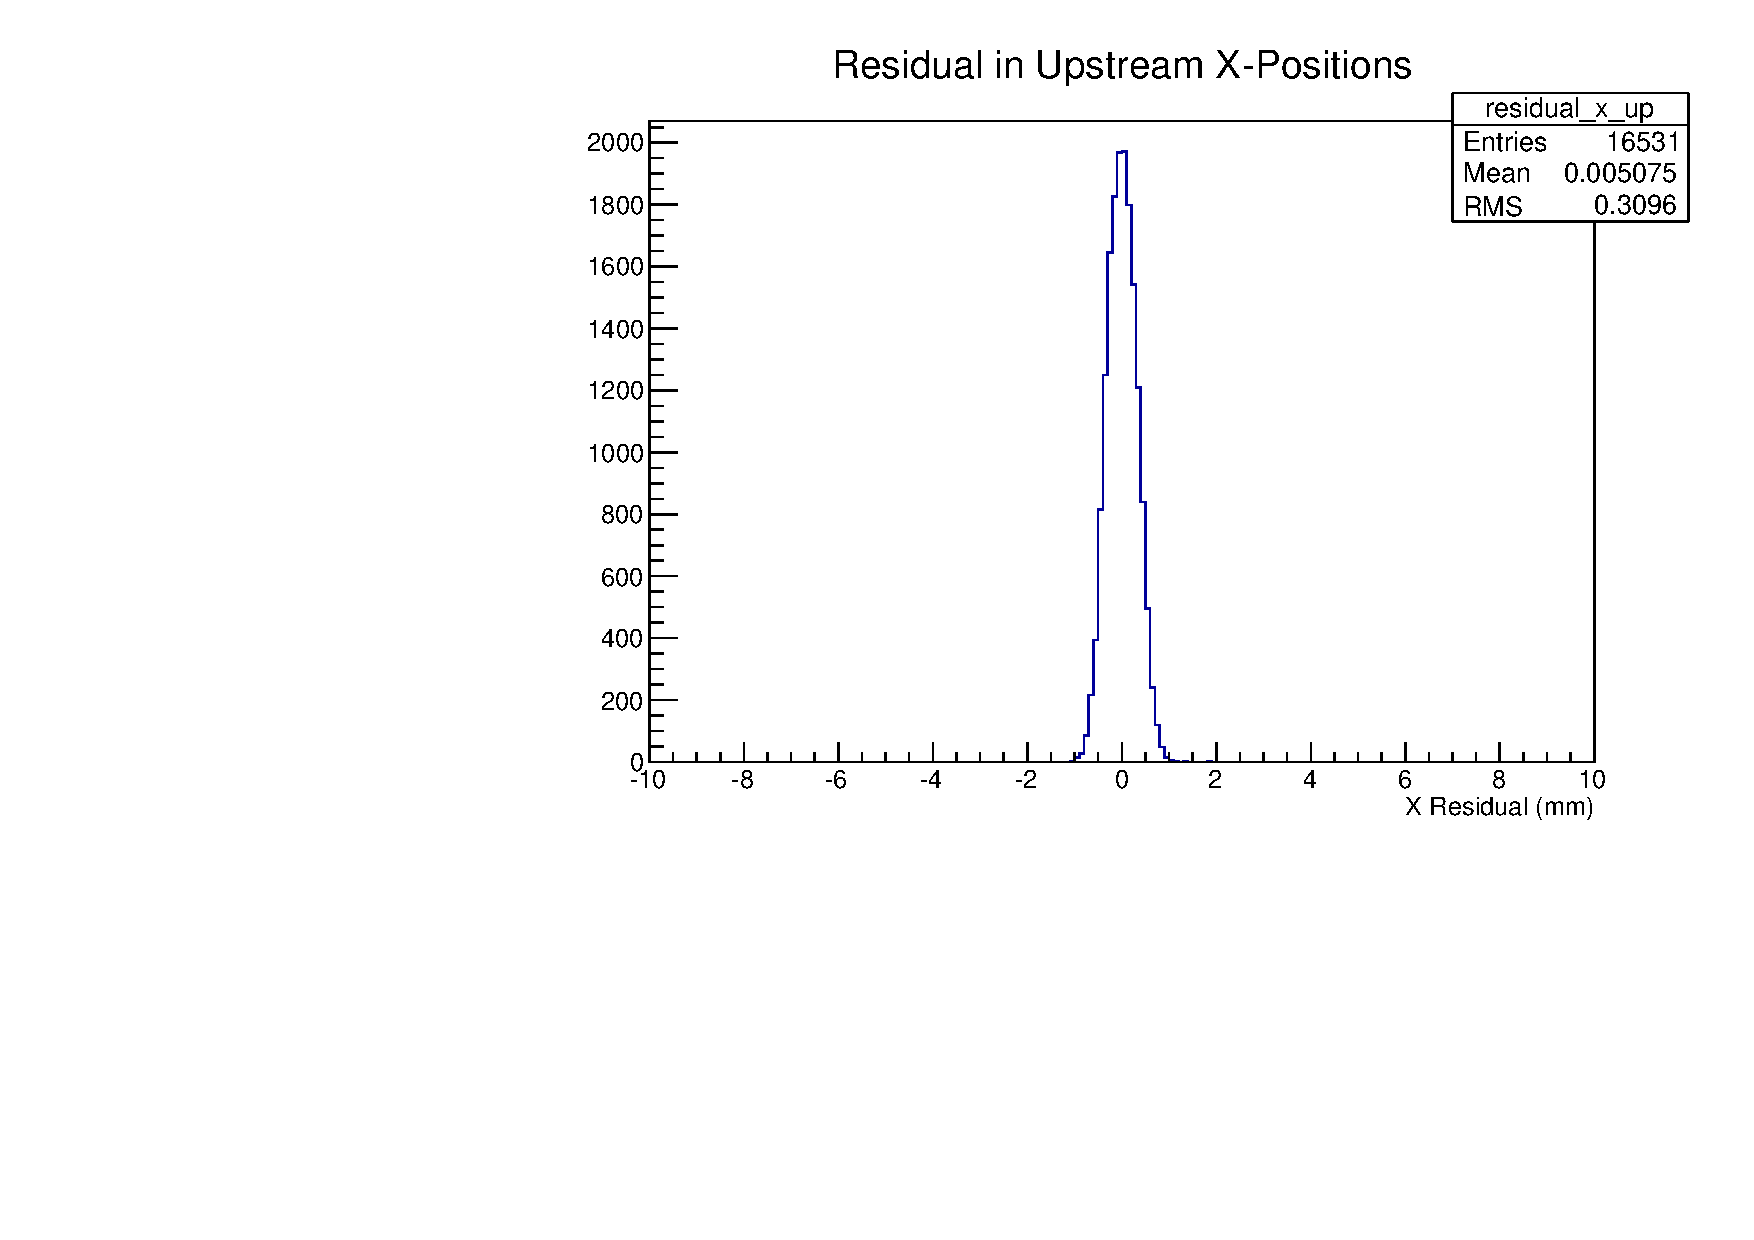
\includegraphics[width=0.49\textwidth, angle=0]{08-Performance/residual_x_up.pdf}
      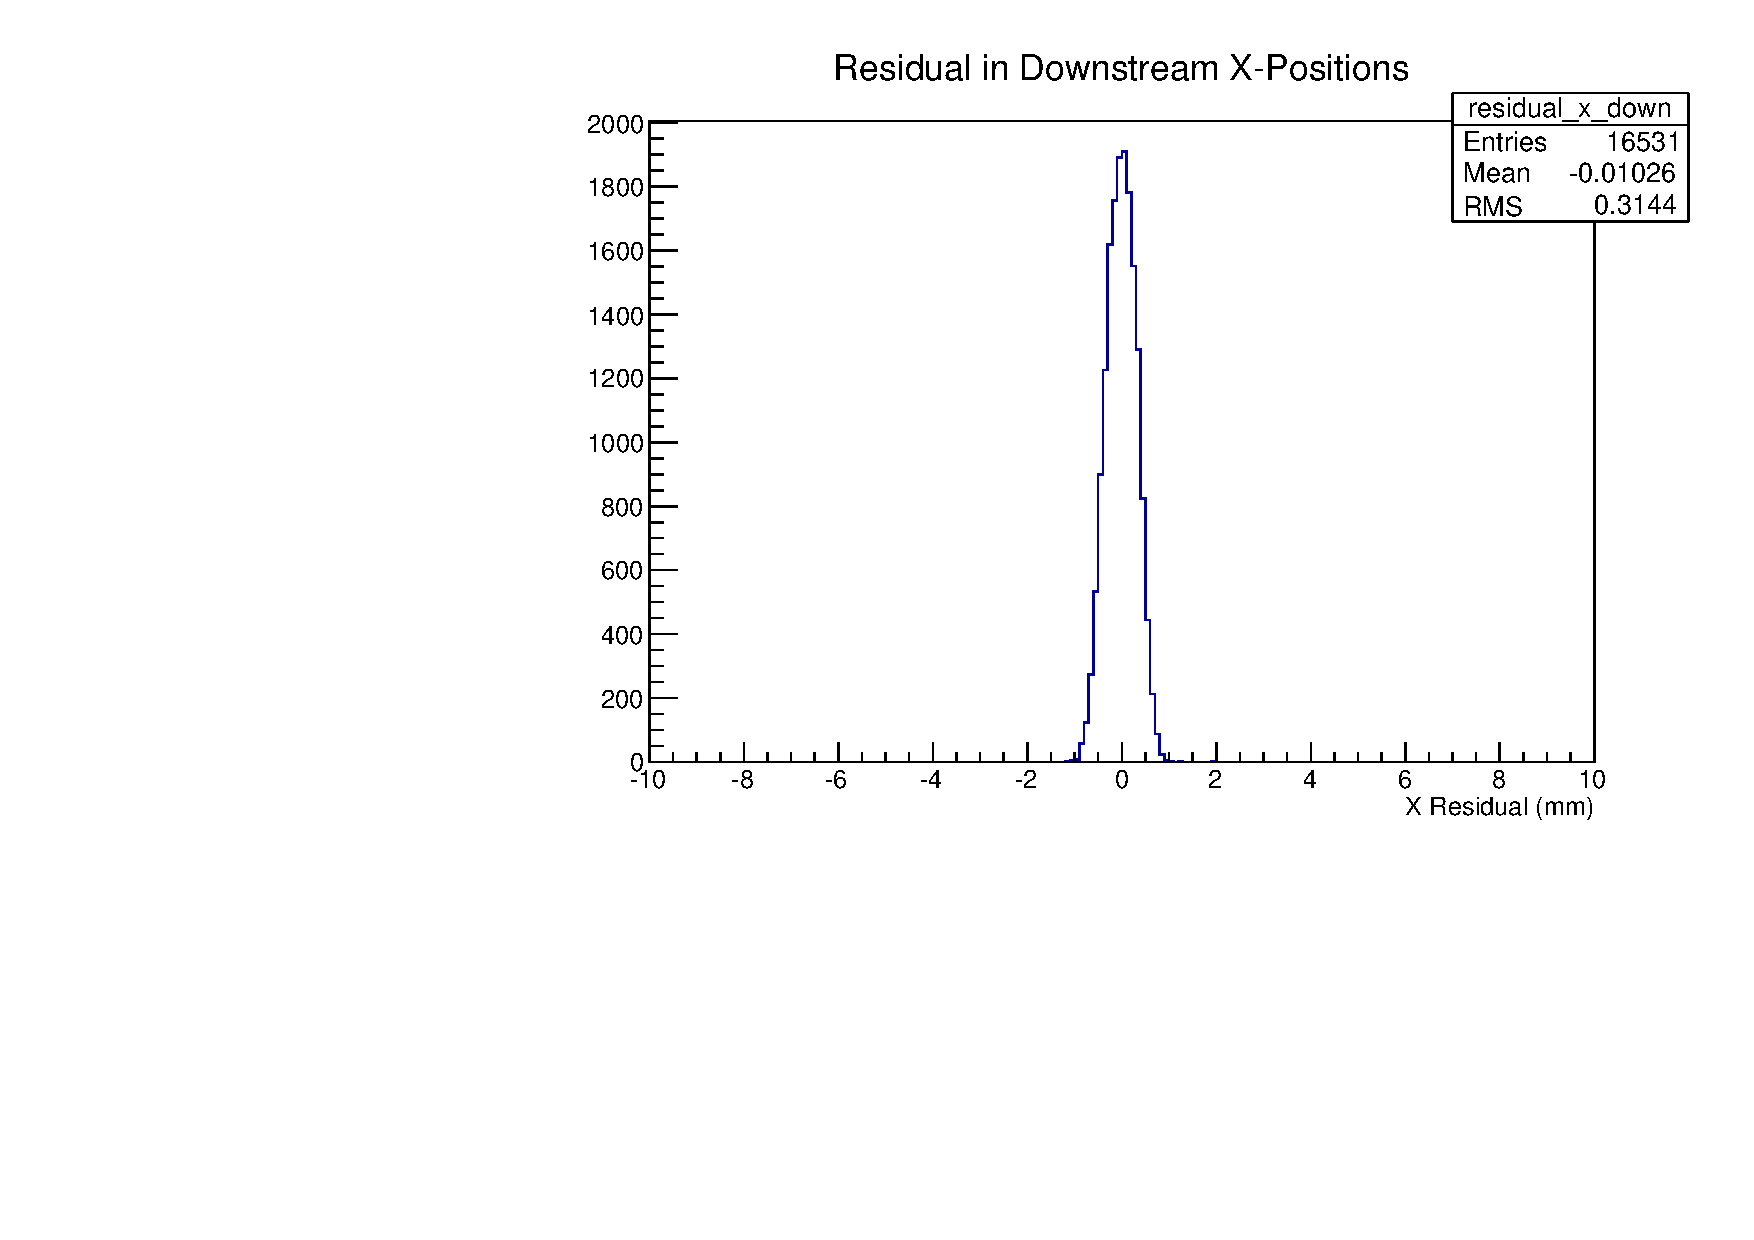
\includegraphics[width=0.49\textwidth, angle=0]{08-Performance/residual_x_down.pdf}
      \caption{\label{fig:XResidKalman} The $x$ residuals of the upstream (left) and downstream (right) trackers for a 6~mm 4D emittance, and 200~MeV/c momentum beam.}
    \end{center}
  \end{figure}
  
    \begin{figure}[p]
    \begin{center}
      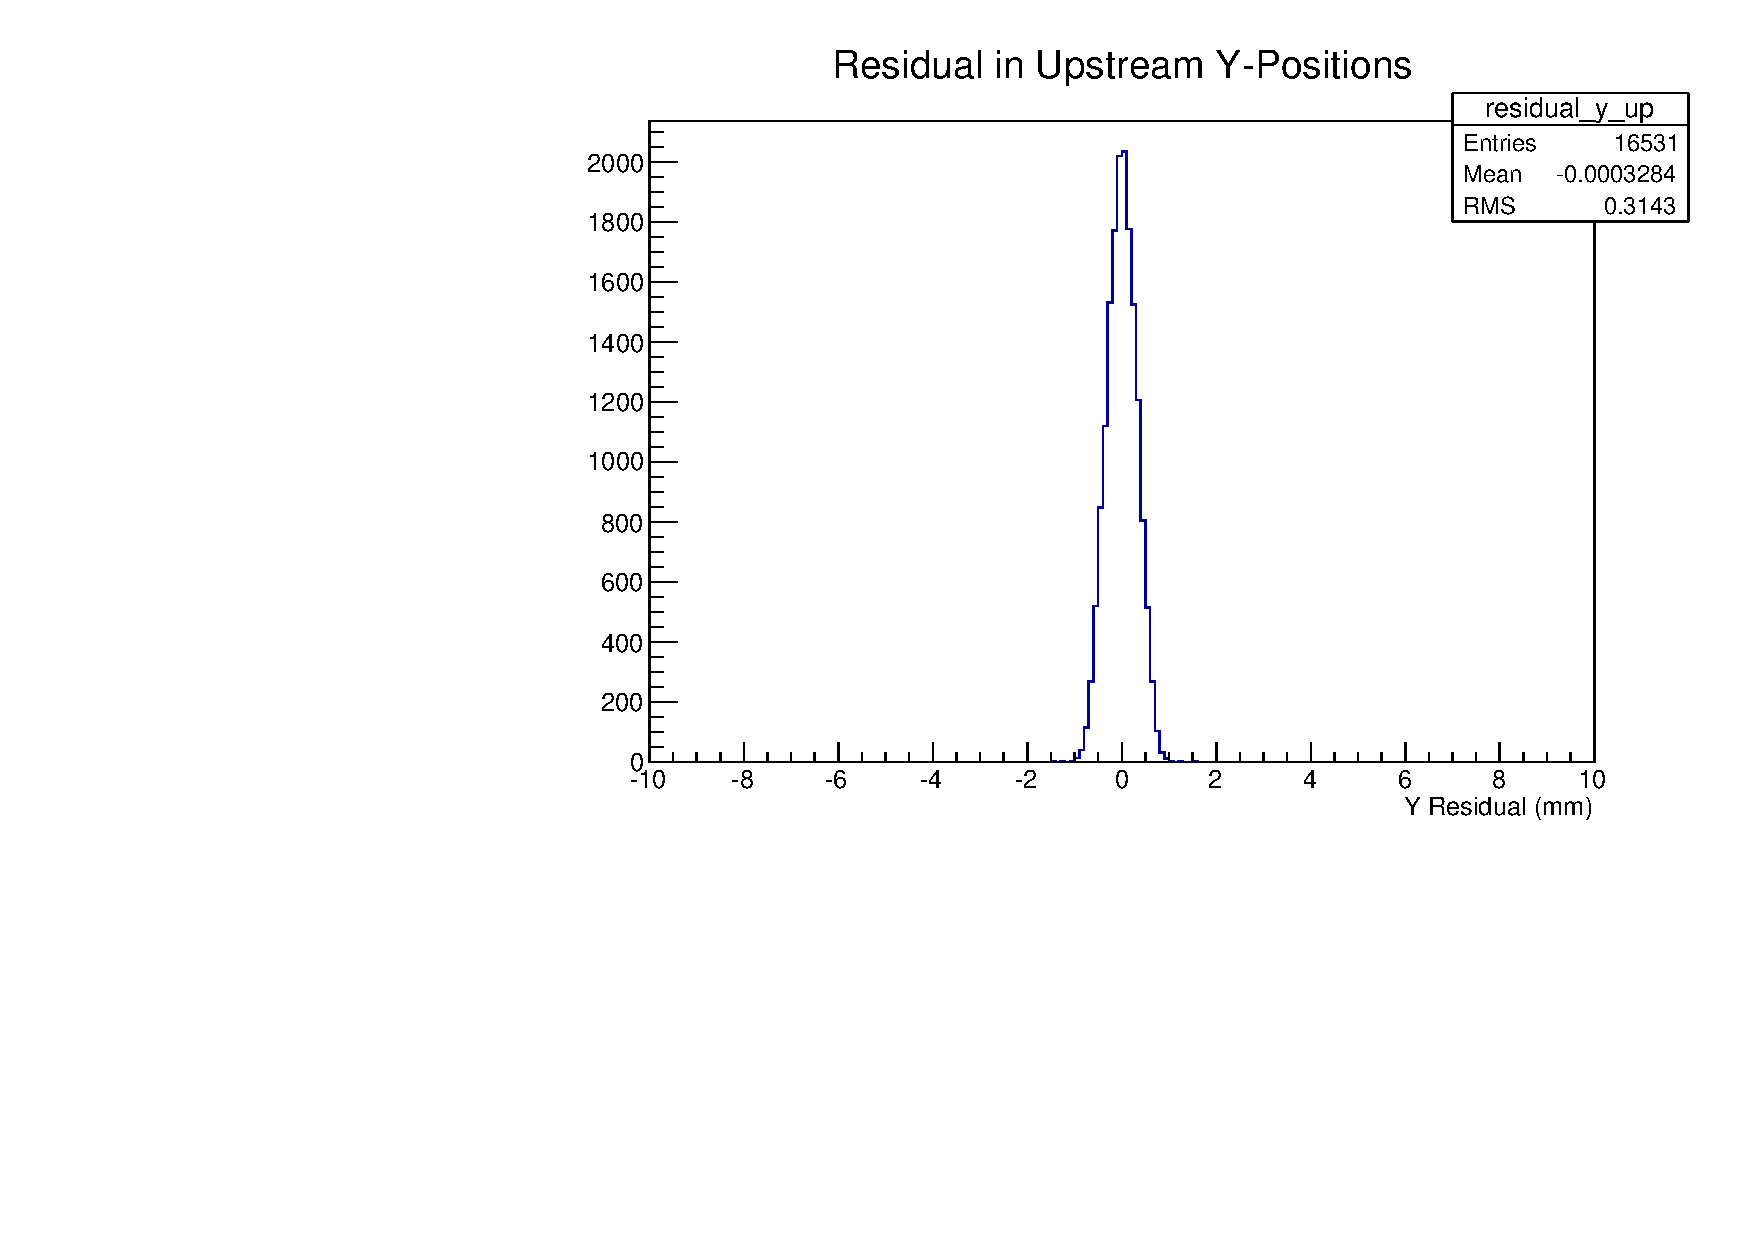
\includegraphics[width=0.49\textwidth, angle=0]{08-Performance/residual_y_up.pdf}
      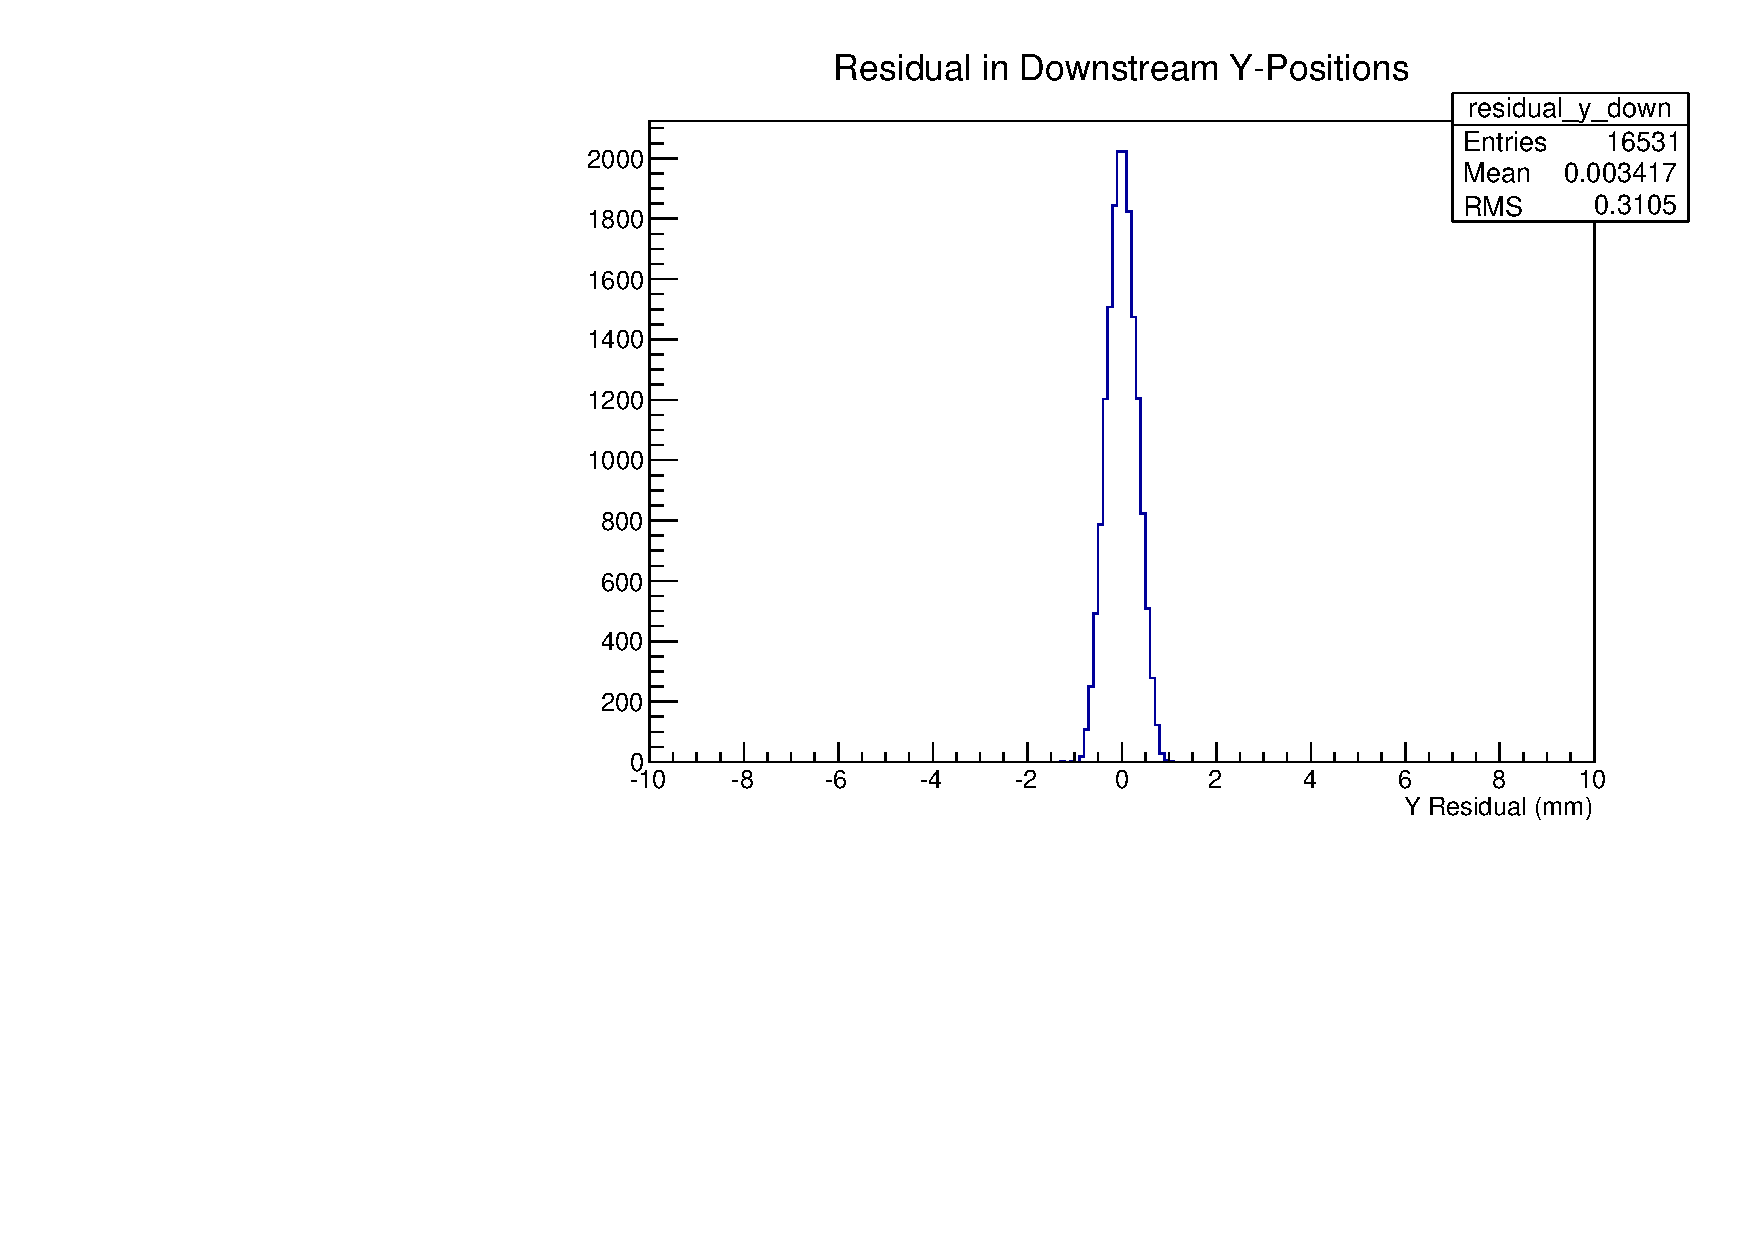
\includegraphics[width=0.49\textwidth, angle=0]{08-Performance/residual_y_down.pdf}
      \caption{\label{fig:YResidKalman} The $y$ residuals of the upstream (left) and downstream (right) trackers for a 6~mm 4D emittance, and 200~MeV/c momentum beam.}
    \end{center}
  \end{figure}
  
  
  \begin{figure}[p]
    \begin{center}
      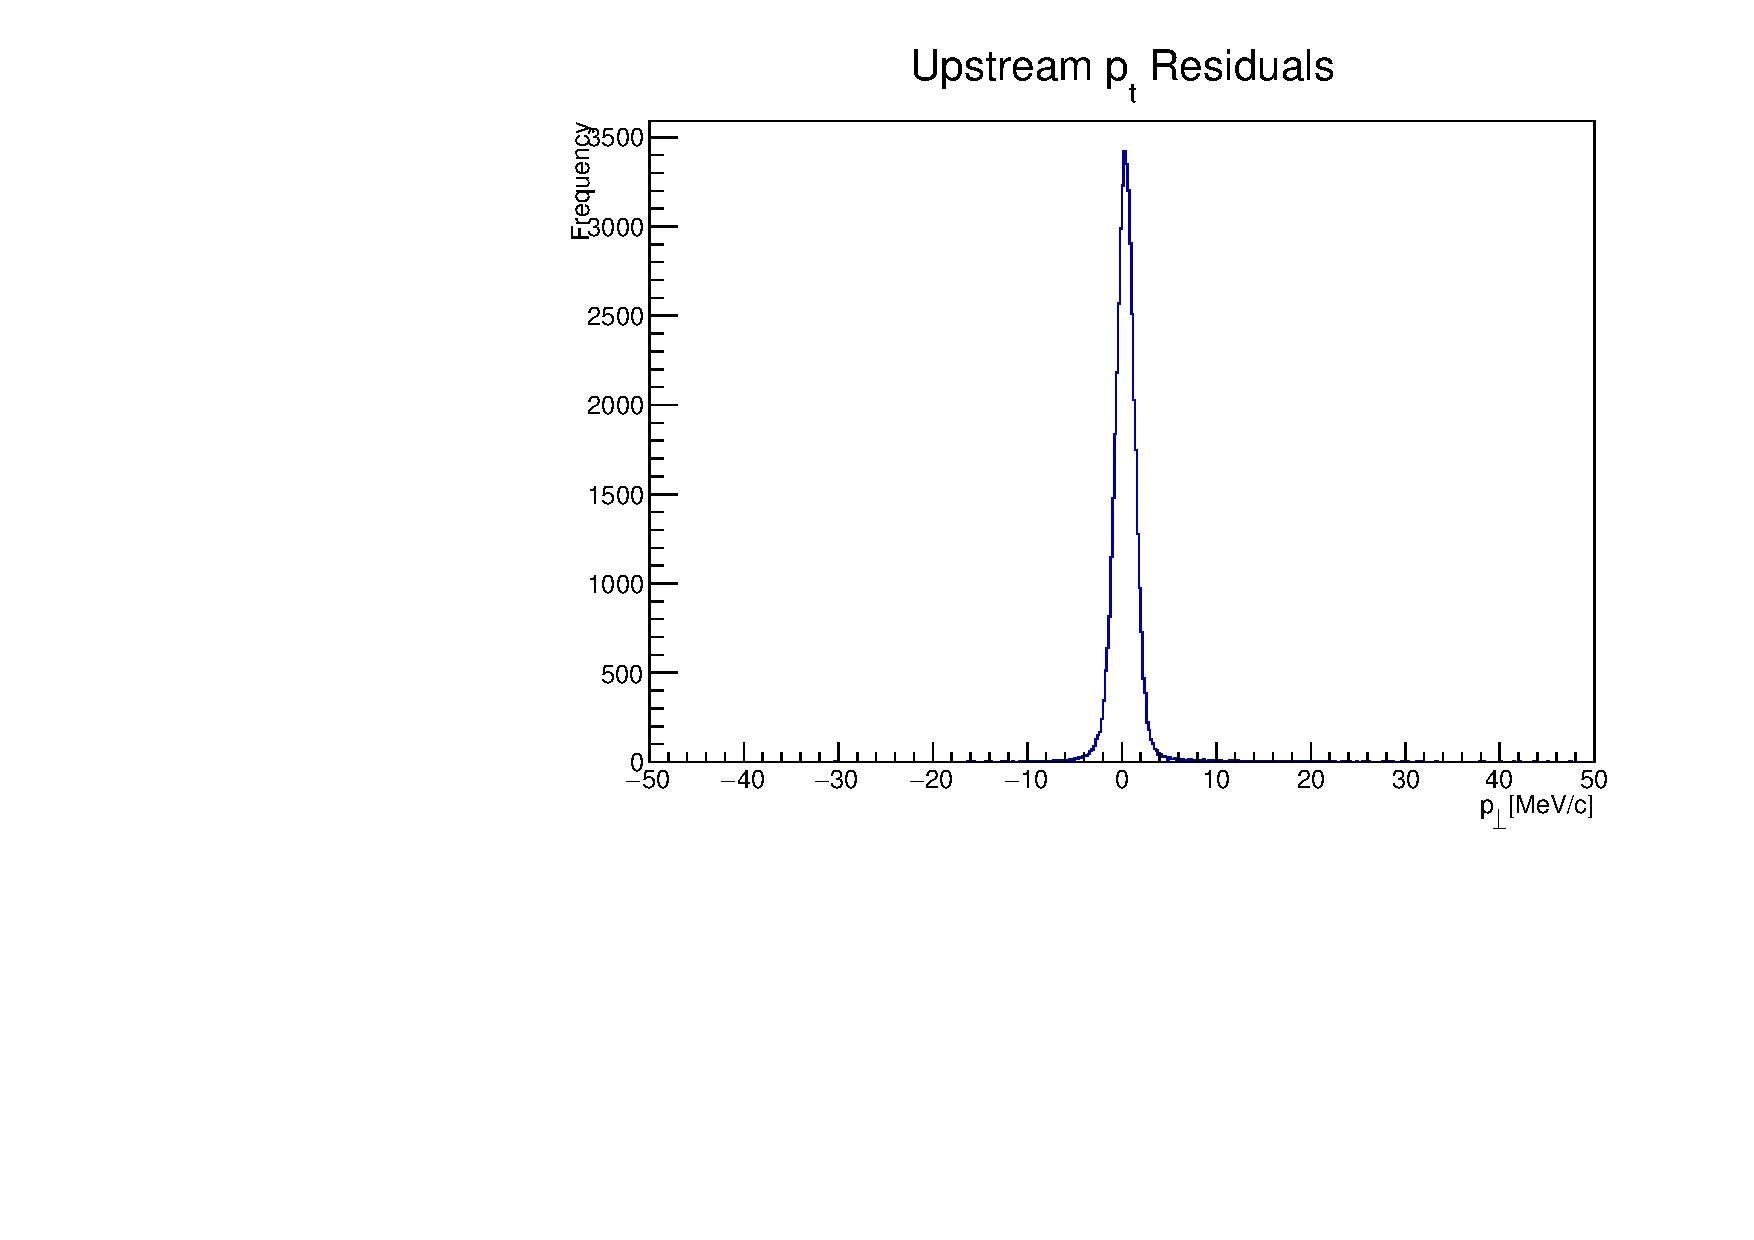
\includegraphics[width=0.49\textwidth, angle=0]{08-Performance/upstream_residual_pt.pdf}
      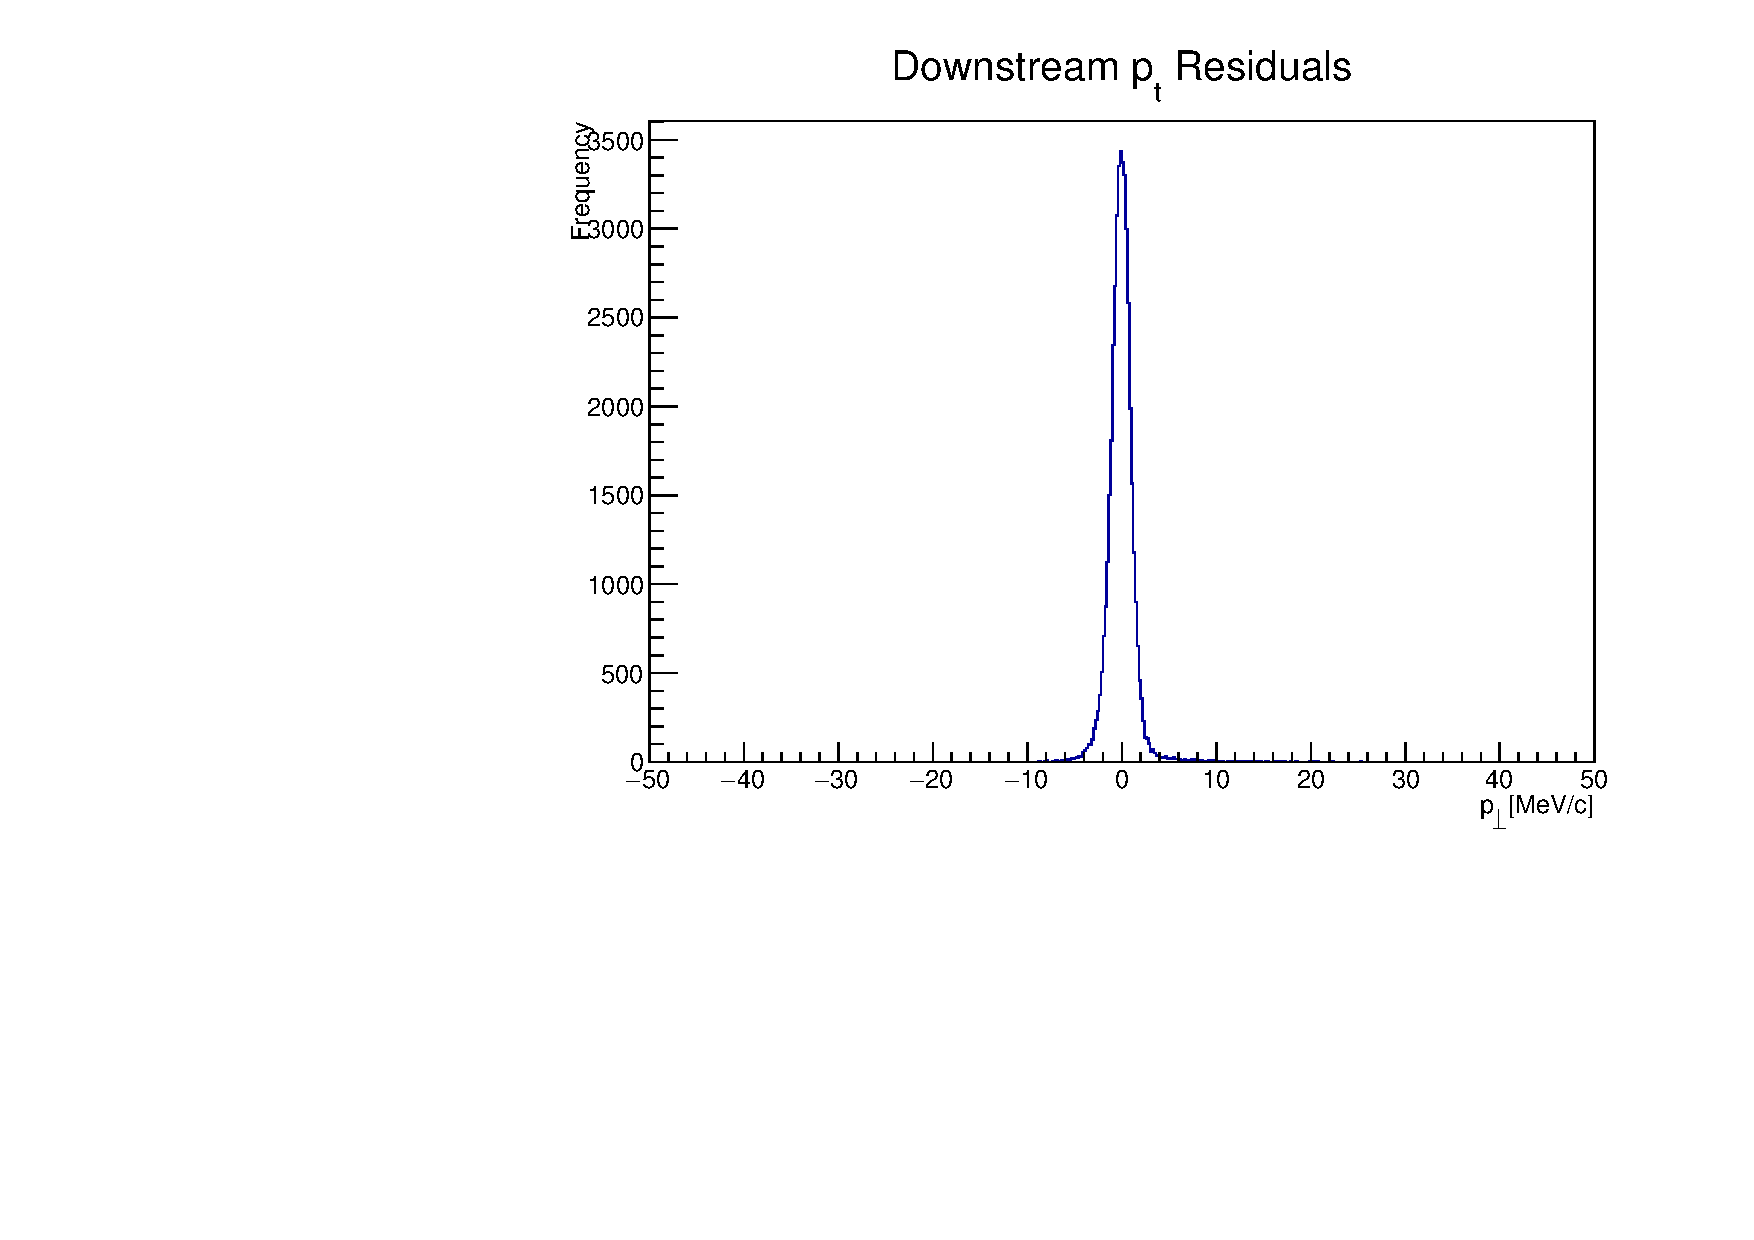
\includegraphics[width=0.49\textwidth, angle=0]{08-Performance/downstream_residual_pt.pdf}
      \caption{\label{fig:PtResidKalman} The $p_t$ residuals of the upstream (left) and downstream (right).}
    \end{center}
  \end{figure}
  
   \begin{figure}[p]
    \begin{center}
      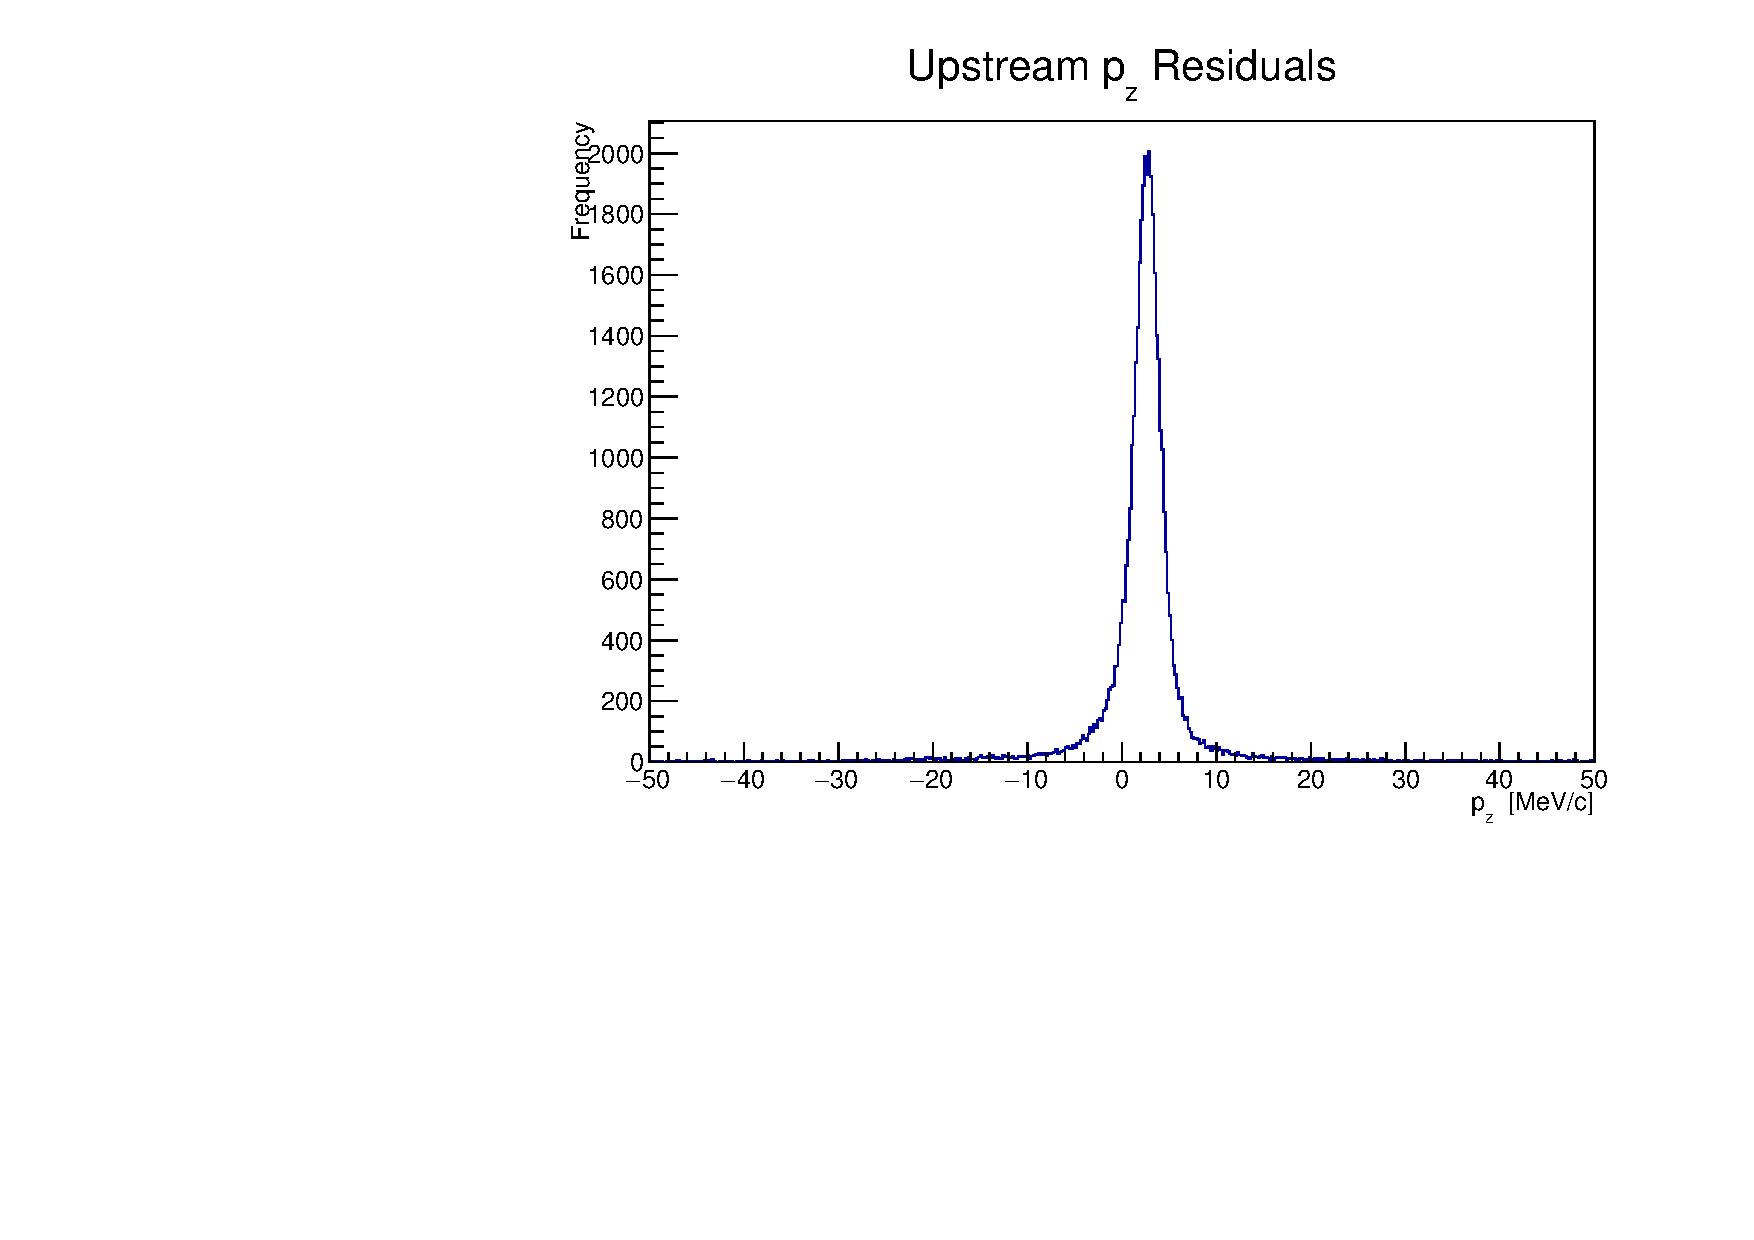
\includegraphics[width=0.49\textwidth, angle=0]{08-Performance/upstream_residual_pz.pdf}
      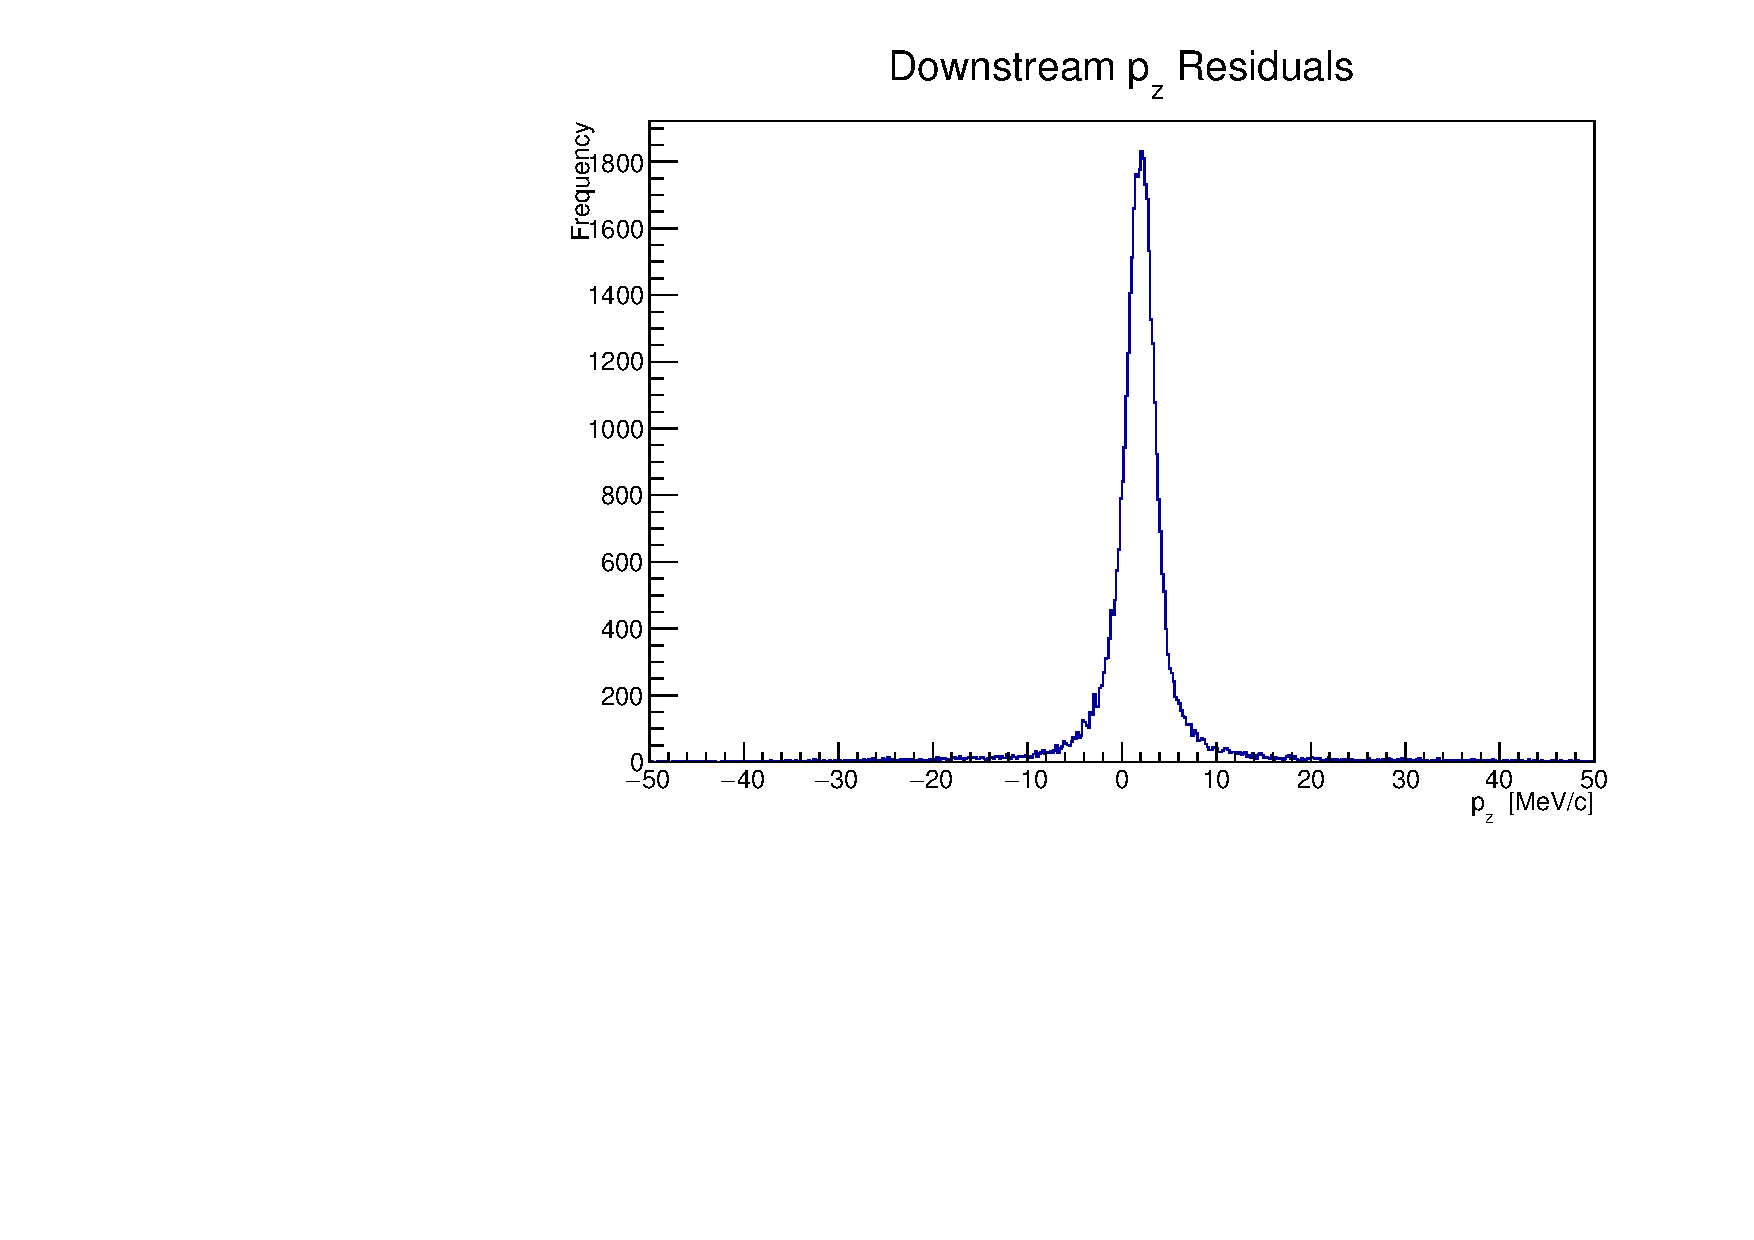
\includegraphics[width=0.49\textwidth, angle=0]{08-Performance/downstream_residual_pz.pdf}
      \caption{\label{fig:PzResidKalman} The $p_z$ residuals of the upstream (left) and downstream (right) trackers for a 6~mm 4D emittance, and 200~MeV/c momentum beam.}
    \end{center}
  \end{figure}
  
  \begin{figure}[p]
   \begin{center}
     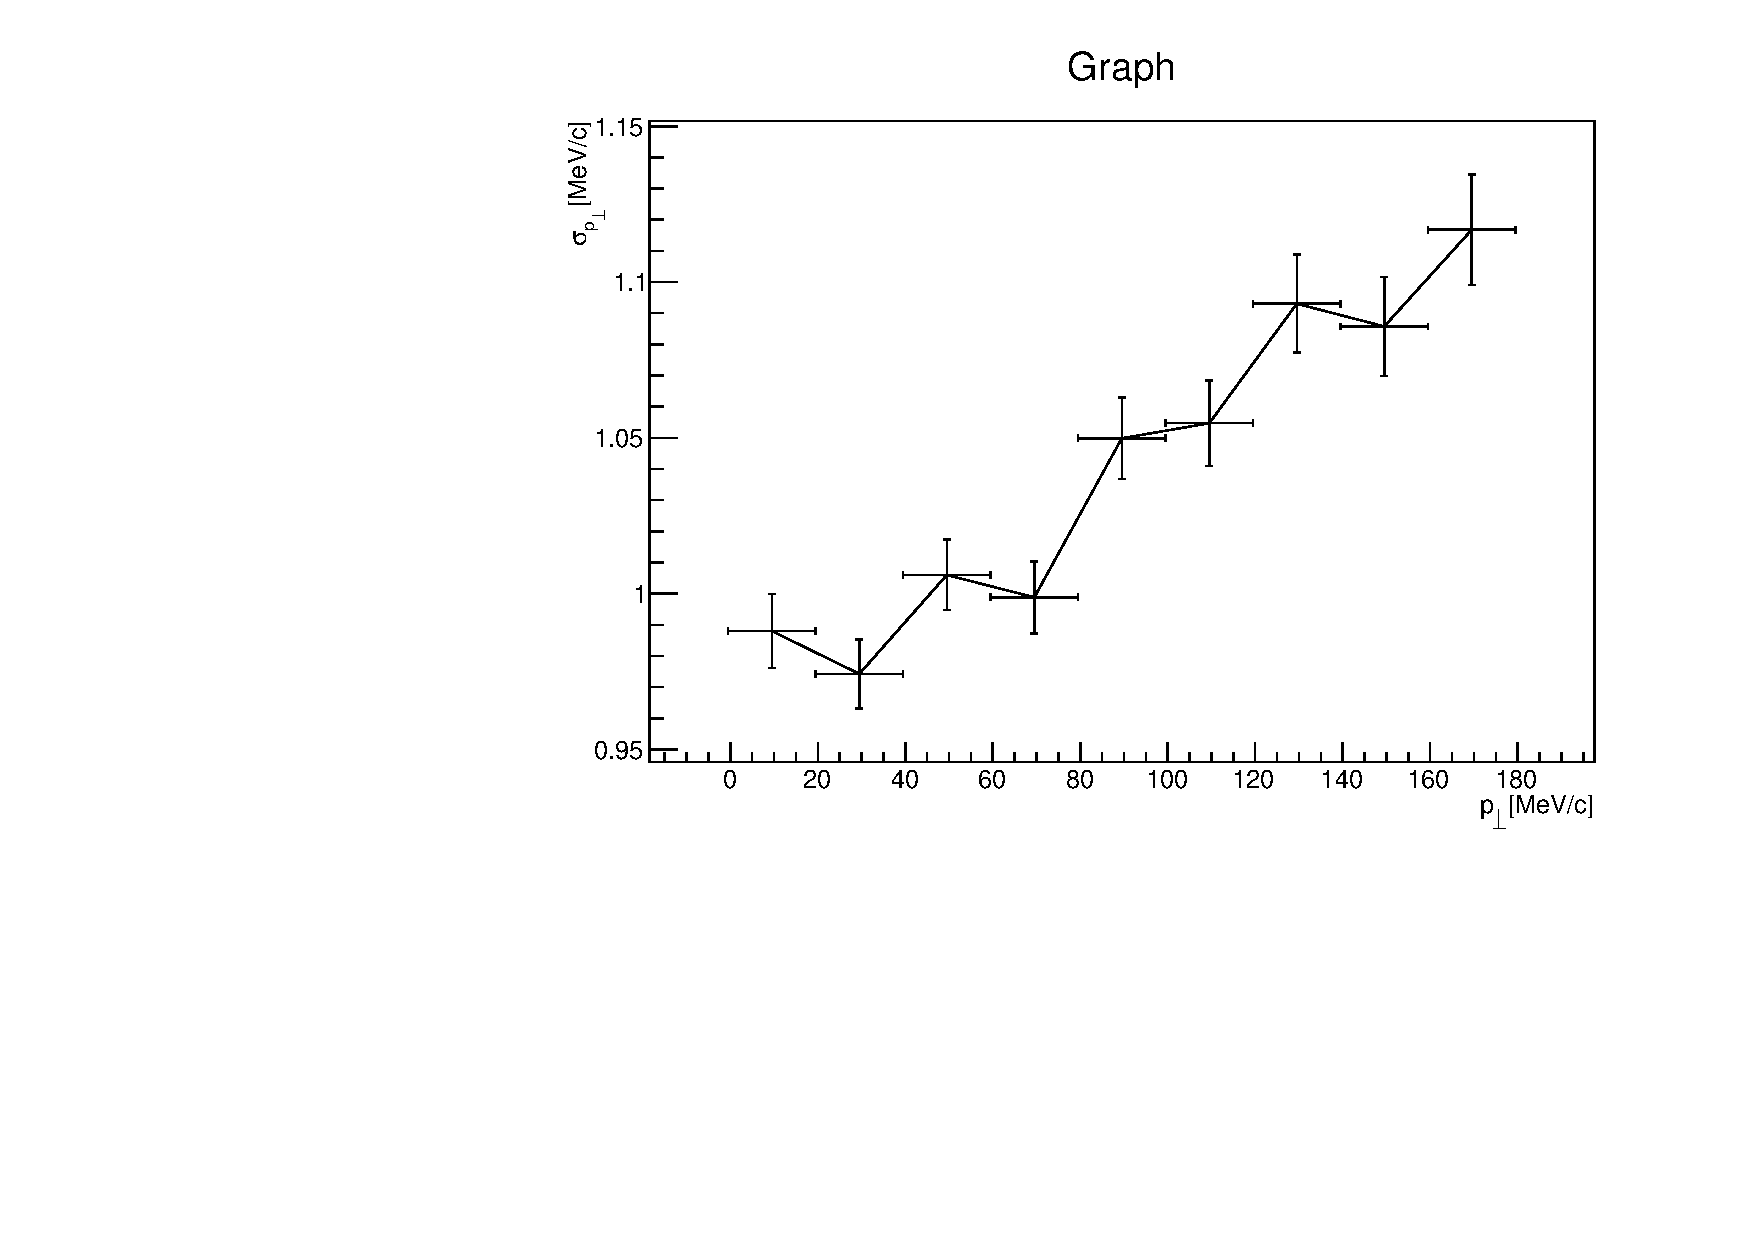
\includegraphics[width=0.49\textwidth, angle=0]{08-Performance/downstream_pt_resolution_vs_pt.pdf}
     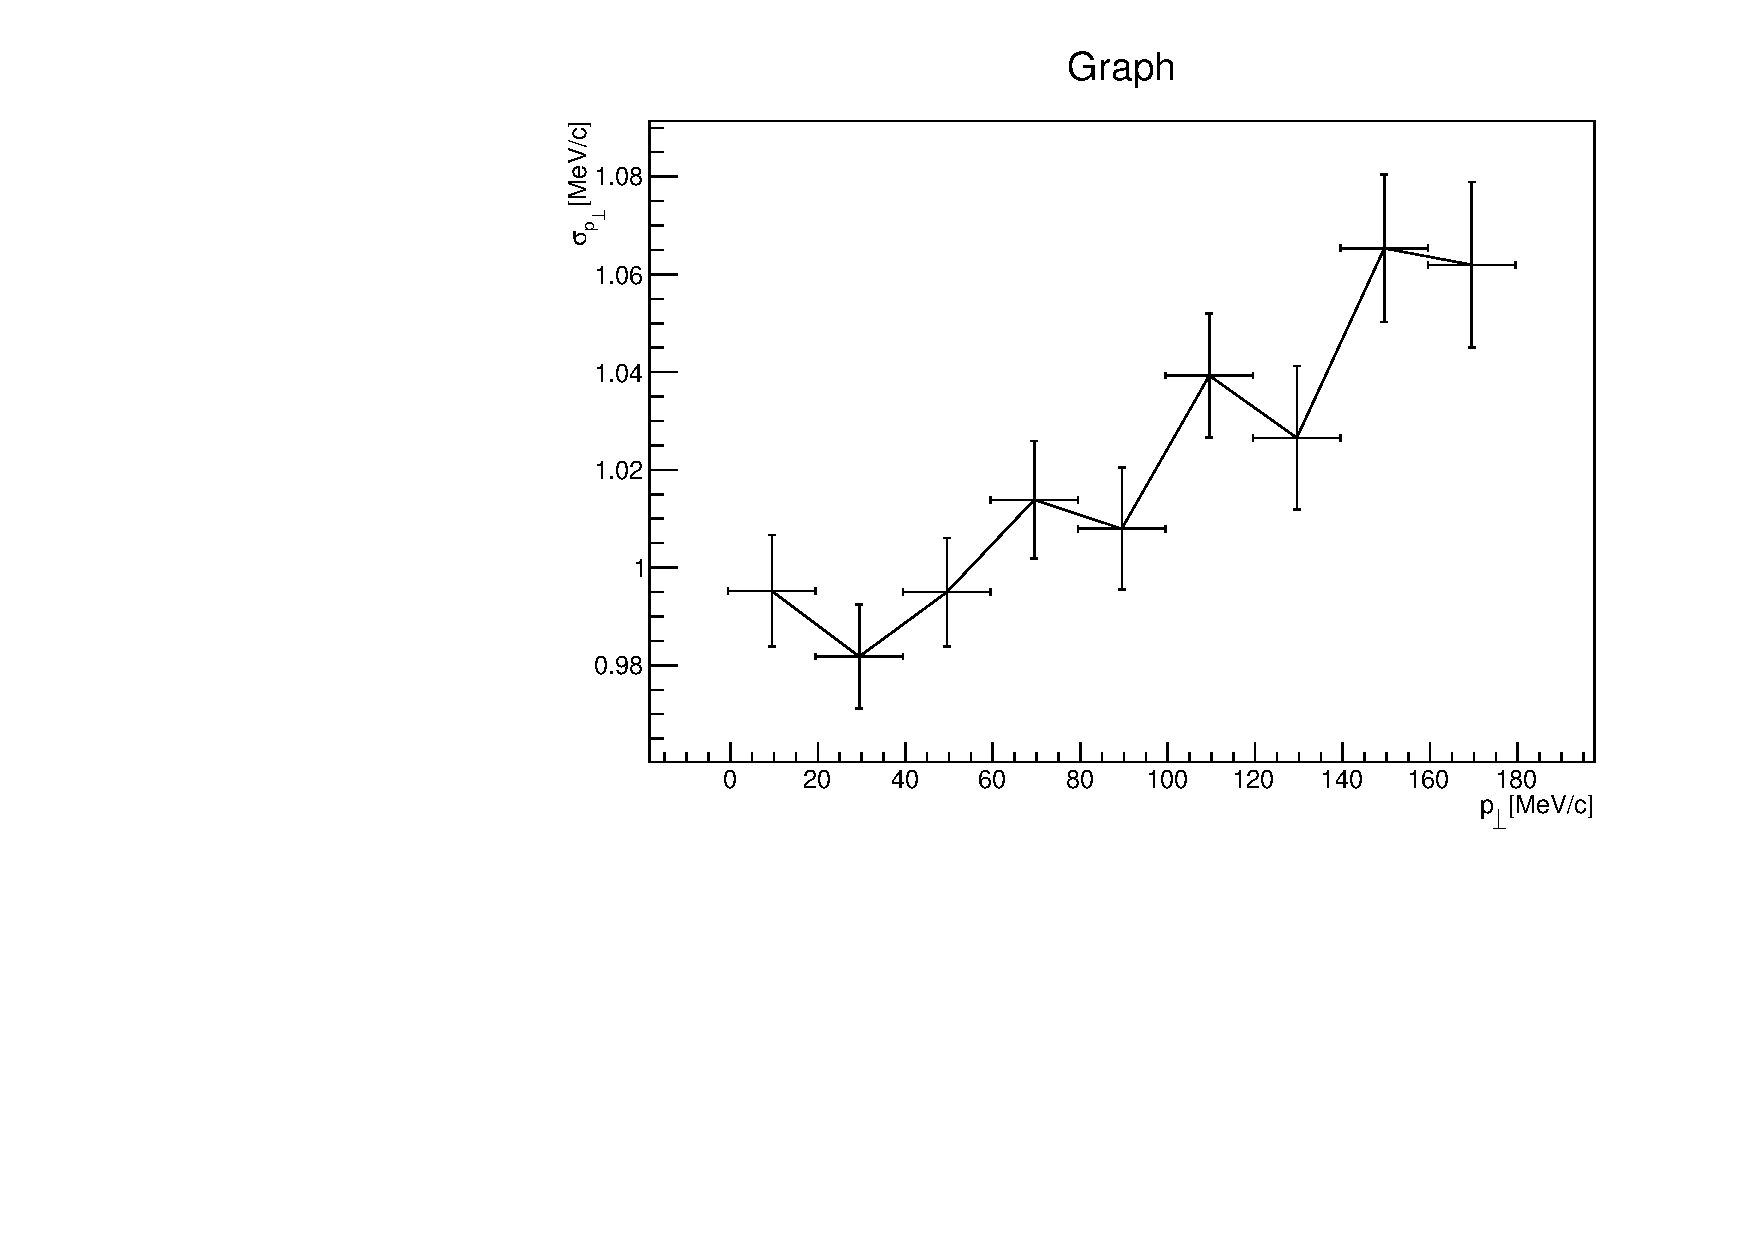
\includegraphics[width=0.49\textwidth, angle=0]{08-Performance/upstream_pt_resolution_vs_pt.pdf}
     \caption{\label{fig:PtPtResolKalman} The $p_t$ resolution vs the $p_t$ of the upstream (left) and downstream (right).}
   \end{center}
  \end{figure}
  
  \begin{figure}[p]
   \begin{center}
     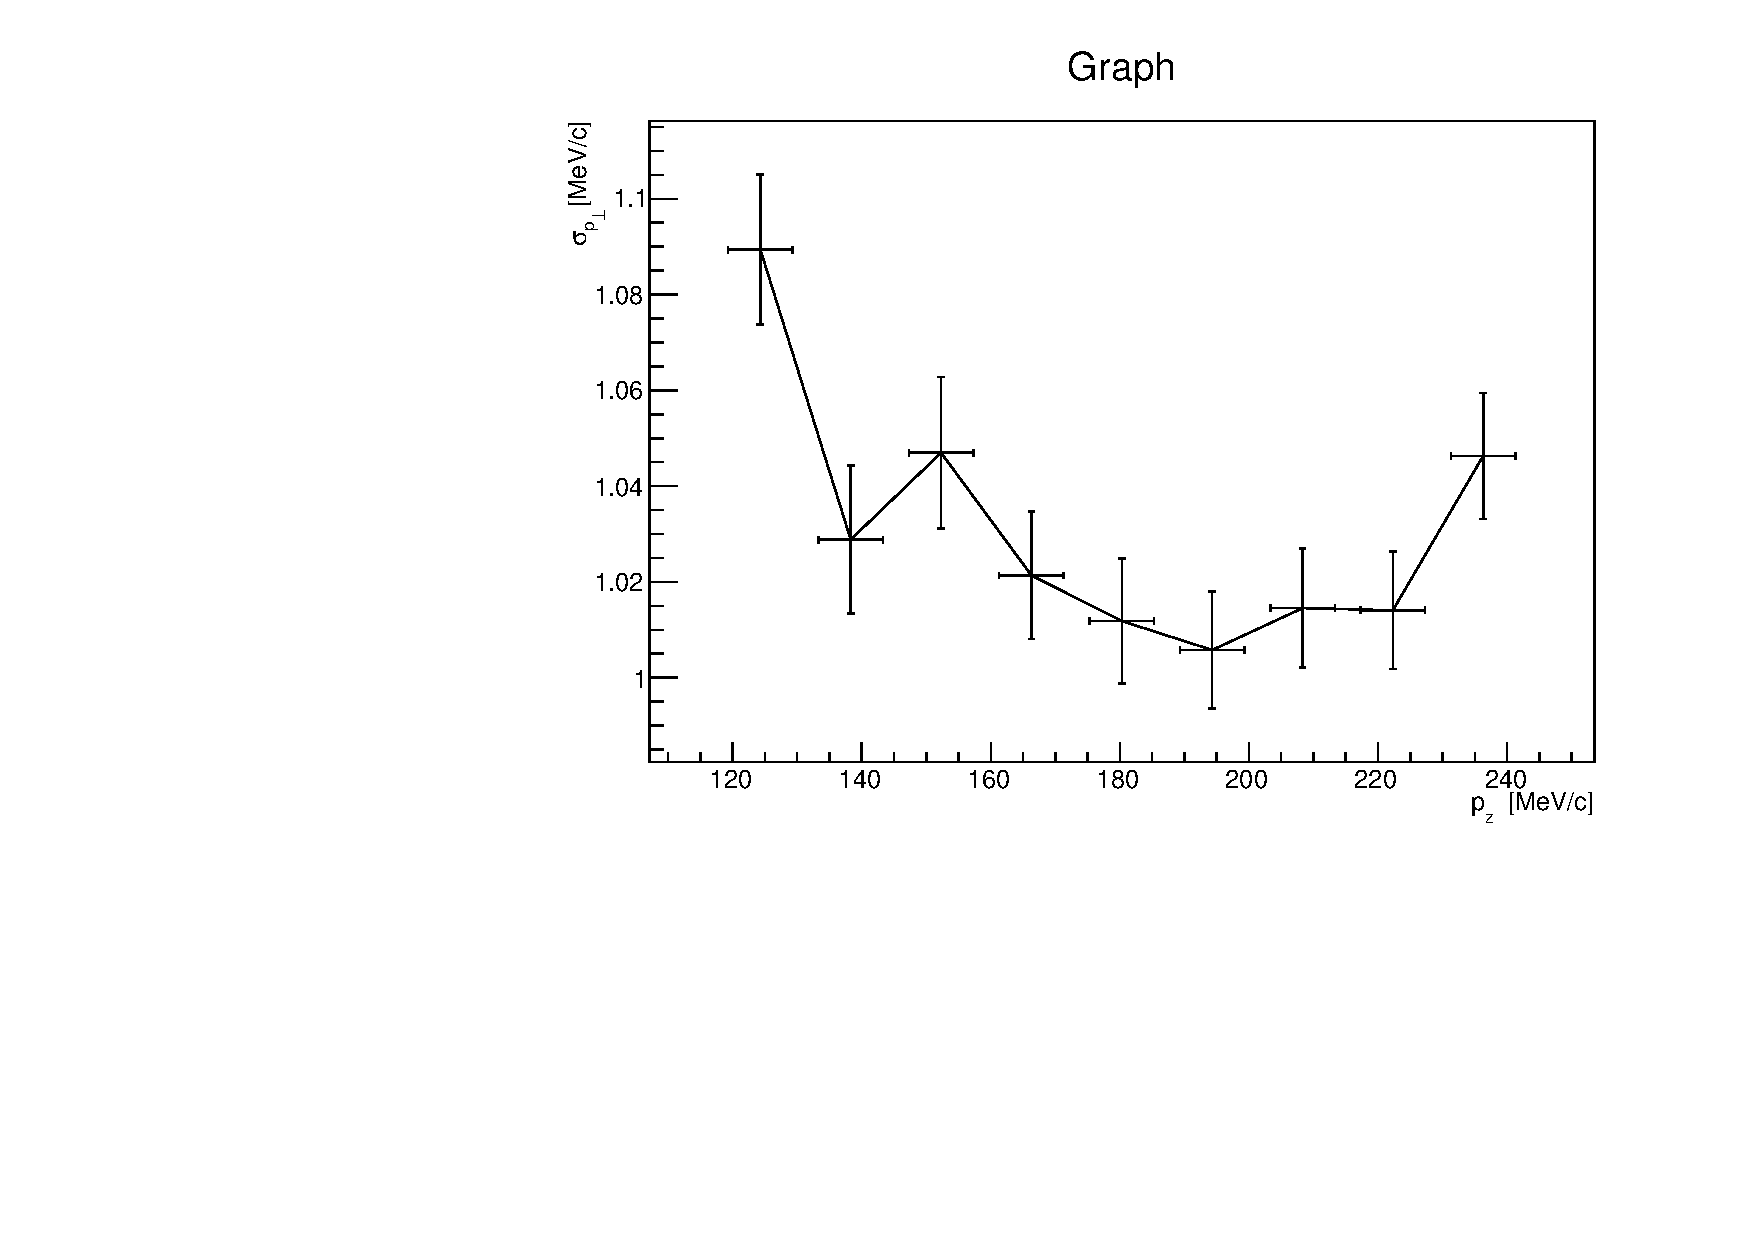
\includegraphics[width=0.49\textwidth, angle=0]{08-Performance/downstream_pz_resolution_vs_pt.pdf}
     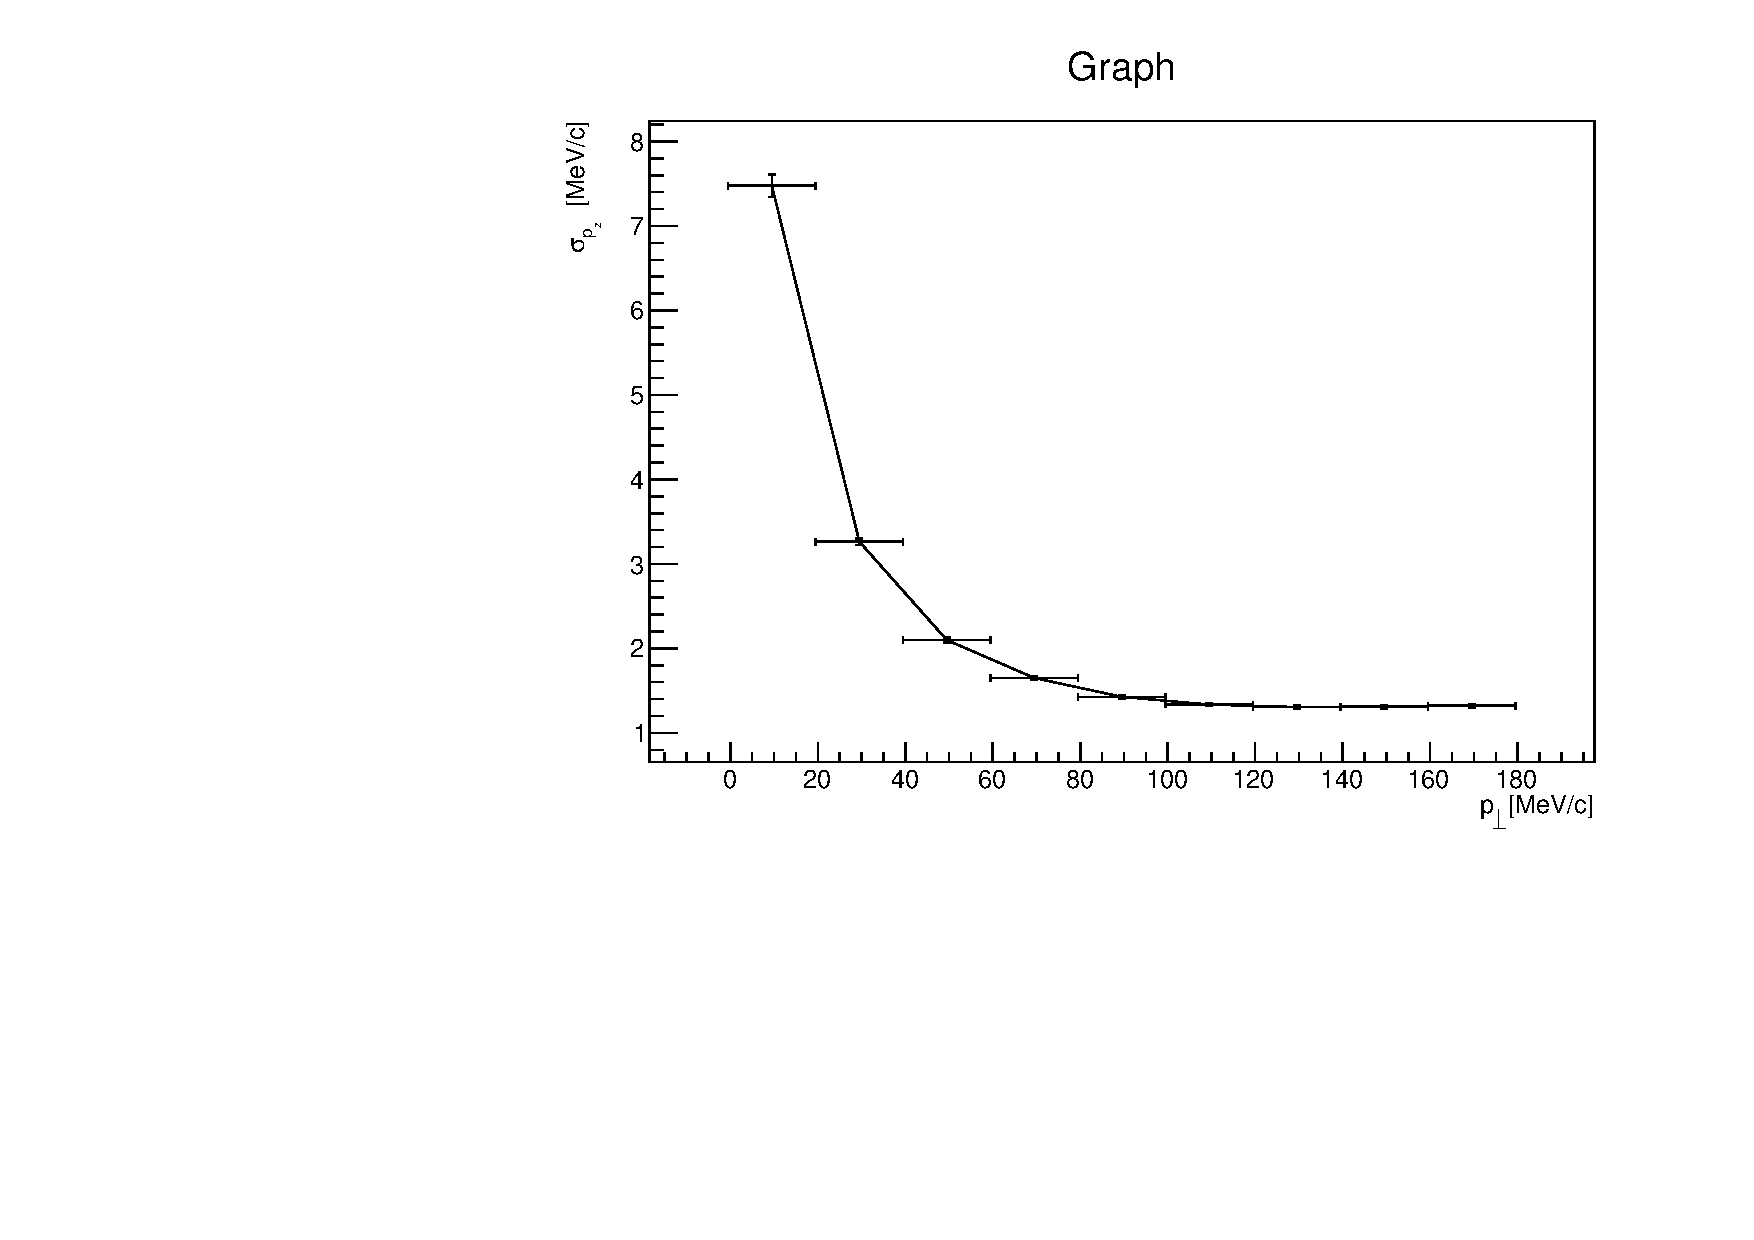
\includegraphics[width=0.49\textwidth, angle=0]{08-Performance/upstream_pz_resolution_vs_pt.pdf}
     \caption{\label{fig:PtPzResolKalman} The $p_z$ resolution vs the $p_t$ of the upstream (left) and downstream (right).}
   \end{center}
  \end{figure}
\section{Conclusion}
\label{sec:Conclusion}

The performance for the final Kalman filter based track fit has been evaluated by comparing Monte Carlo truth with reconstructed data, for the key tracker measurements of $x$, $y$, $p_{\perp}$ and $p_z$.  The observed performance in the transverse position and momentum measurements is excellent, for both the upstream and downstream trackers. A systematic offset in $p_z$ requires further investigation, though the resolution remains acceptable.

Future Monte Carlo studies will evaluate the performance of the MICE emittance measurement and how the resolutions of the trackers could bias the measurements.


\clearpage

\bibliography{MICE_2014-05}                                                                           
\bibliographystyle{99-Styles/utphys}


% \cleardoublepage
% \appendix
% \input 11-AuthorList/11-AuthorList

\end{document}
